%%%%%%%% NeurIPS 2026 SUBMISSION FILE %%%%%%%%%%%%%%%%%

\documentclass{article}

% NeurIPS 2026 style file (anonymous submission with line numbers).
\usepackage{neurips_2026}
% For arXiv preprint, use
% \usepackage[preprint]{neurips_2026}
% For camera-ready, use
% \usepackage[final]{neurips_2026}

\usepackage[utf8]{inputenc}
\usepackage[T1]{fontenc}
\usepackage{microtype}
\usepackage{graphicx}
\usepackage{subcaption}
\usepackage{booktabs} % for professional tables
\usepackage{hyperref}
\usepackage{url}
\usepackage{xcolor}
\usepackage{algorithm}
\usepackage{algorithmic}

% Attempt to make hyperref and algorithmic work together better:
\providecommand{\theHalgorithm}{\arabic{algorithm}}

% Provide \yrcite fallback (it is defined by icml2026.sty but not by
% neurips_2026.sty); behave like \citeyear so existing source compiles.
\providecommand{\yrcite}[1]{\citeyear{#1}}

\usepackage{amsmath}
\usepackage{amssymb}
\usepackage{amsfonts}
\usepackage{nicefrac}
\usepackage{mathtools}
\usepackage{amsthm}
\usepackage{tikz}


% if you use cleveref..
\usepackage[capitalize,noabbrev]{cleveref}

%%%%%%%%%%%%%%%%%%%%%%%%%%%%%%%%
% THEOREMS
%%%%%%%%%%%%%%%%%%%%%%%%%%%%%%%%
\theoremstyle{plain}
\newtheorem{theorem}{Theorem}[section]
\newtheorem{proposition}[theorem]{Proposition}
\newtheorem{lemma}[theorem]{Lemma}
\newtheorem{corollary}[theorem]{Corollary}
\theoremstyle{definition}
\newtheorem{definition}[theorem]{Definition}
\newtheorem{assumption}[theorem]{Assumption}
\theoremstyle{remark}
\newtheorem{remark}[theorem]{Remark}

%%% cref setting.
\crefname{assumption}{Assumption}{Assumptions}
\crefname{figure}{Fig{.}}{Figs{.}}%{Figures}
\crefname{table}{Tab{.}}{Tabs{.}}
\crefname{definition}{Definition}{Definitions}
\crefname{theorem}{Theorem}{Theorems}
\crefname{lemma}{Lemma}{Lemmas}
\crefname{proposition}{Proposition}{Propositions}
\crefname{corollary}{Corollary}{Corollaries}
\crefname{problem}{Problem}{Problems}
\crefname{example}{Example}{Examples}
\crefname{fact}{Fact}{Facts}
\crefname{conjecture}{Conjecture}{Conjectures}
\crefname{remark}{Remark}{Remarks}
\crefname{condition}{Condition}{Conditions}
\crefname{requirement}{Requirement}{Requirements}
\crefname{enumi}{}{}
%% \crefname{equation}{Eq.}{Eqs.}
\crefname{equation}{Eq{.}}{Eqs{.}}
%% \crefname{section}{{\S}}{{\S}}
\crefformat{section}{\S#2#1#3}
\crefmultiformat{section}{\S#2#1#3}{ and~\S#2#1#3}{, \S#2#1#3}{, and~\S#2#1#3}
% Todonotes is useful during development; simply uncomment the next line
%    and comment out the line below the next line to turn off comments
%\usepackage[disable,textsize=tiny]{todonotes}
\usepackage[textsize=tiny]{todonotes}

\newcommand*{\fix}{\marginpar{FIX}}
\newcommand*{\new}{\marginpar{NEW}}
\newcommand*{\TODO}[1]{\textcolor{red}{\textbf{[TODO: }#1\textbf{]}}}
\newcommand*{\tk}[1]{\textcolor{olive}{\textbf{[TK : }#1\textbf{]}}}
\newcommand*{\hy}[1]{\textcolor{blue}{\textbf{[HY : }#1\textbf{]}}}
\newcommand*{\jb}[1]{\textcolor{orange}{\textbf{[JB : }#1\textbf{]}}}
\newcommand*{\jl}[1]{\textcolor{purple}{\textbf{[JL : }#1\textbf{]}}}


\newcommand*{\threewidth}{0.25\textwidth}
\newcommand*{\threeimagewidth}{0.9\textwidth}
\newcommand*{\twowidth}{0.225\textwidth}
\newcommand*{\twoimagewidth}{0.9\textwidth}

\newcommand*{\R}{\mathbb{R}}
\newcommand*{\Z}{\mathbb{Z}}
\renewcommand{\thempfootnote}{\arabic{mpfootnote}}

\title{Implicit Neural Representations\\ for Variational Problems on Graphons}

% Authors are anonymized at submission time; the NeurIPS style hides them
% unless the [final] option is selected.
\author{%
  Anonymous Authors\\
  Affiliation \\
  \texttt{anonymous@example.com}
}

\begin{document}

\maketitle

\allowdisplaybreaks

\begin{abstract}
We propose a neural exploratory framework for \emph{continuous variational problems over graphons}, i.e., symmetric measurable functions $[0,1]^2 \to [0,1]$ that arise as limits of dense graph sequences. Such problems are central to two parts of the mathematical literature: extremal graph theory, which studies graph parameter optimisation under given restrictions, often for those graphs with a large number of vertices, and the large deviation theory of dense random graphs, which characterises typical large-deviation events through constrained graphon optimisation. We represent graphons by implicit neural networks and optimise graphon objectives by gradient descent. Our design combines three ingredients: a multi-scale sinusoidal residual architecture biased toward sharp, step-like graphons; an embedded solver that enforces a single empirical density constraint and is differentiated by implicit differentiation; and symmetry-aware Monte Carlo estimators. On generalised Tur\'an problems and density-domination problems that previously required substantial human effort, the framework rediscovers known optimal graphons without human intervention. Applied to open instances, it produces candidate optima, including a previously unreported family of extremal structures. The same architecture and training loop, with only a change of constraint and objective, also handle the upper-tail variational problem governing large deviations for triangle counts in Erd\H{o}s--R\'enyi random graphs.
\end{abstract}


\section{Introduction} \label{sec:introduction}

Machine learning is opening new directions in mathematical discovery. Recent work spans automatic provers and autoformalisation for Olympiad-style problems~\citep{polu2023formal, trinh2024solving, jiang2023draft, wu2022autoformalization, deepmind2024alphaproof, huang2025gemini}, neural search for combinatorial constructions~\citep{adam2021constructions, charton2024patternboost, romera2024mathematical, novikov2025alphaevolve}, and pattern-driven progress on long-standing conjectures in pure mathematics~\citep{davies2021advancing, he2024murmurations}. In this paper we extend this line of research to a class of \emph{continuous variational problems over graphons}, with three motivating instances drawn from extremal graph theory and large deviation theory of dense random graphs.

A central object in extremal graph theory is the \emph{homomorphism density} $t(H, G)$ between finite undirected graphs $H$ and $G$: the probability that a uniformly random map from $V(H)$ to $V(G)$ is a graph homomorphism. As a basic example, the constrained optimisation problem
\begin{equation}
  \max_G\, t(K_2, G)
  \quad\text{ subject to }\quad
  t(K_3, G) = 0 \;\land\; |V(G)| = n
  \label{eqn:mantel}
\end{equation}
asks for an $n$-vertex triangle-free graph that maximises the edge density. Here $K_m$ denotes the complete graph on $m$ vertices, so $K_2$ and $K_3$ represent an edge and a triangle, respectively. Although the answer is given by the classical theorem of Mantel~\yrcite{mantel1907vraagstuk}, a large family of similar problems involving homomorphism densities remain open~\citep{sidorenko1993correlation, borgs2006counting, razborov2008minimal}.

A standard approach to such problems is to study their \emph{asymptotic} counterparts, taking $n \to \infty$ and analysing the limit of the optimum. These asymptotic problems can often be reformulated as continuous optimisation over \emph{graphons}: symmetric measurable functions $[0,1]^2 \to [0,1]$ that arise as limit objects of dense graph sequences~\citep{lovasz2012large}. Another source of graphon variational problems comes from the large deviation theory of dense random graphs~\citep{chatterjee2011large}, where the limiting structure of an Erd\H{o}s--R\'enyi graph conditioned on an unusually large subgraph density is itself characterised by a constrained optimisation over graphons. In both settings, the objective and constraints are integrals against the graphon $W$ (homomorphism densities or pointwise relative entropy), and known or conjectured optima are step-like.

We attack these graphon problems directly with deep learning, representing $W$ as a neural network in the spirit of implicit neural representations~\citep{park2019deepsdf,mescheder2019occupancy,chen2019learning} and minimising the objective by gradient descent on the network parameters. Three recurring challenges shape our design. First, known and conjectured optima are typically step-like, and standard architectures struggle with such targets because of their bias toward smooth functions. We address this with a \emph{multi-scale sinusoidal residual architecture} that injects sinusoidal encodings of growing frequency into successive layers, biasing the model toward sharp, step-like solutions. Second, both the objective and the constraints are graphon integrals that must be estimated from samples, including the high-dimensional homomorphism-density integrals; we use symmetry-aware Monte Carlo estimators. Third, the problems often carry a single scalar density constraint (a fixed edge density, or a fixed triangle density) that is poorly handled by penalty terms; we embed a numerical solver for an empirical version of the constraint into the forward pass and backpropagate through it via implicit differentiation, as in deep equilibrium models~\citep{bai2019deep}.

We evaluate this single framework on three classes of graphon variational problems that share these characteristics but originate in distinct mathematical contexts: \textbf{(P1)} generalised Tur\'an problems, minimising a homomorphism density under a fixed edge-density constraint; \textbf{(P2)} density-domination problems, testing whether one homomorphism density (raised to an integer power) dominates another; and \textbf{(P3)} the upper-tail variational problem of \citet{chatterjee2011large}, minimising a relative-entropy functional under a fixed triangle-density constraint. On \textbf{(P1)} and \textbf{(P2)}, our framework rediscovers nontrivial known optima that previously required substantial human effort~\citep{goodman1959on,bollobas1975relations,lovasz1983on,fisher1989lower,razborov2008minimal}, produces candidate minimisers for open instances such as $7$-cycle density, identifies candidate violations of clique-density inequalities, and through a systematic sweep over small graphs, uncovers a previously unreported family of extremal structures for a six-vertex graph that does not match the complete $k$-partite pattern of classical examples. On \textbf{(P3)}, the same architecture, solver, and training loop apply with only a change of objective and of the  constraint type, providing a uniform handle on a problem class whose optimisers describe the conditional structure of Erd\H{o}s--R\'enyi graphs in their upper-tail regime.
We view the framework as a flexible exploratory tool that complements rigorous lower-bound techniques such as flag algebras~\citep{razborov2007flag,falgas2013applications}: it produces candidate upper bounds, concrete candidate minimisers, and structural conjectures that can be inspected, refined, or subsequently certified.

\section{Background} \label{sec:background}

For a positive integer $n$, write $[n] \coloneqq \{1,2,\ldots,n\}$. Throughout the paper, a \emph{graph} is an undirected, finite, simple graph (no self-loops and no multiple edges). For a graph $G$, we write $V(G)$ and $E(G)$ for its vertex and edge sets, and let $v(G) \coloneqq |V(G)|$ and $e(G) \coloneqq |E(G)|$. We use standard notation for familiar graphs: $K_n$ denotes the complete graph on $n$ vertices (with vertex set $[n]$ and edge set $\{\{i,j\} : i, j \in [n],\, i \neq j\}$), and $C_n$ denotes the cycle on $n$ vertices (with vertex set $[n]$ and edge set $\{\{i,i+1\} : 1\le i\le n-1\} \cup \{\{n,1\}\}$).

Let $H$ and $G$ be graphs. A \emph{homomorphism} from $H$ to $G$ is a map $\phi : V(H) \to V(G)$ that preserves adjacency, i.e., $\{\phi(u), \phi(v)\} \in E(G)$ for every $\{u,v\} \in E(H)$. The \emph{homomorphism density} from $H$ to $G$, denoted $t(H, G)$, is the probability that a uniformly random map $\phi : V(H) \to V(G)$ is a homomorphism. Equivalently,
\begin{align}
t(H, G) \,\coloneqq\, {}
\label{eqn:homomorphismdensity}
\frac{1}{v(G)^{v(H)}}
\!\!
\sum_{\phi : V(H) \to V(G)}
\prod_{\{u,v\} \in E(H)} \mathbb{I}\bigl[\{\phi(u), \phi(v)\} \in E(G)\bigr],
\end{align}
where $\mathbb{I}[\cdot]$ is the indicator function.
Homomorphism densities are a natural language for extremal graph problems: they are size-normalised statistics of fixed patterns, so objectives and constraints are comparable across graphs of different sizes, and they are central to dense graph limit theory, quasirandomness, and regularity-based approximation~\citep{lovasz2012large}.

A \emph{graphon} $W$ is a symmetric measurable function $W : [0,1]^2 \to [0,1]$. Intuitively, $W$ can be viewed as the (probabilistic) adjacency matrix of a continuum graph with vertex set $[0,1]$: $W(x,y)$ is the probability of an edge between $x$ and $y$. Graphons arise as limits of dense graphs. Along any graph sequence whose homomorphism densities $t(F, G_n)$ converge for every fixed graph $F$ with vertex set $[v(F)]$, there is a graphon $W$ with $t(F, G_n) \to t(F, W)$ for every $F$, where
$t(F,W)$ is the graphon homomorphism density of $F$ in $W$ defined by
\begin{align}
t(F, W) \,\coloneqq\, \mathbb{E}_{x_1, \ldots, x_{v(F)} \stackrel{\mathrm{iid}}{\sim} \mathrm{Unif}[0,1]}
\Big[ \prod_{\{i,j\} \in E(F)} W(x_i, x_j)\Big].
\label{eqn:homomorphismdensitygraphon}
\end{align}
Conversely, every graphon arises in this way~\citep{lovasz2012large}. Familiar discrete structure is reflected in $W$: balanced complete bipartite graphs converge to the two-block graphon equal to $1$ on the off-diagonal blocks and $0$ on the diagonal blocks; an Erd\H{o}s--R\'enyi $G(n,q)$ converges to the constant graphon $W \equiv q$; a stochastic block model converges to a multi-block graphon whose blocks correspond to the communities. 

Graphons provide a common language for all three problem classes studied in this paper: the objective and constraints in each involve graphon homomorphism densities $t(H,W)$ or closely related graphon integrals, and the structure of the optimisers is the central object of interest. The first two classes arise from extremal graph theory, where optimising over graphons is equivalent to optimising the corresponding asymptotic finite-graph problem~\citep{lovasz2012large}; the third arises from large deviation theory of dense random graphs. We describe each in turn.

\paragraph{Constrained density minimisation.}
The first task is to minimise the homomorphism density of a fixed graph $H$ subject to a fixed edge density $p$. Because the edge density of a finite graph takes only certain rational values, we phrase the asymptotic extremal problem in terms of graph sequences:
\begin{equation}
\label{eqn:extremalproblem:generalisedTuran}
\inf\Big\{\liminf_{n \to \infty} t(H, G_n) \,\Big|\, \text{$(G_n)$ is a graph sequence with } v(G_n)\to\infty \text{ and } t(K_2, G_n)\to p\Big\}.
\end{equation}
By the graph-limit theory~\citep{lovasz2012large}, this equals $\min_{W:\,t(K_2,W)=p}\, t(H, W)$, the graphon problem our method optimises directly.
This generalises Tur\'an's theorem~\citep{Turan1941}
and the Erd\H{o}s--Stone--Simonovits theorem~\citep{erdos1946on, erdos1966limit}, both classical results in extremal graph theory,
which say that for every $H$ and $p \leq 1 - 1/(\chi(H) - 1)$, where $\chi(H)$ is the chromatic number of $H$, the optimum is $0$. But for $p > 1 - 1/(\chi(H) - 1)$, the problem is much harder, and complete solutions are known only for a handful of $H$: $H = K_r$ for all $r \ge 3$~\citep{reiher2016clique}, with landmark earlier results for $r = 3$~\citep{razborov2008minimal} and $r = 4$~\citep{nikiforov2011number}; and for $C_5$, the solution is known only for $p = 1 - 1/k$ ($k$ a positive integer)~\citep{bennet2020minimizing}.

\paragraph{Density inequalities.}
The second task asks whether the inequality $t(H_1, G)^{m_2} \geq t(H_2, G)^{m_1}$ holds asymptotically for all graphs $G$, for given graphs $H_1, H_2$ and positive integers $m_1, m_2$. Again by the graph-limit theory~\citep{lovasz2012large}, this reduces to asking whether the graphon optimum
\begin{equation}
\label{eqn:extremalproblem:dominationExponent}
\min_{W}\,\bigl( t(H_1, W)^{m_2} - t(H_2, W)^{m_1} \bigr)
\end{equation}
is non-negative.
Sidorenko's conjecture~\citep{sidorenko1992, sidorenko1993correlation} predicts non-negativity when $H_1$ is bipartite, $H_2 = K_2$, and $(m_1, m_2) = (e(H_1), 1)$ (so the expression reduces to $t(H_1,W) - t(K_2,W)^{e(H_1)}$), and more systematic studies of general pairs $(H_1, H_2)$ appear in recent work~\citep{conlonlee2024domination, behague2025}.

\paragraph{Variational problem from large deviation theory.}
Large deviation theory for random graphs addresses two related questions: at what exponential rate does $G(n,q)$ produce an atypically large subgraph density, and what does the graph typically look like when such a rare event occurs?
These questions are of fundamental interest in probability theory and combinatorics, and they carry information-theoretic structure that is natural from an ML perspective: the Chatterjee--Varadhan framework reduces both questions to a single constrained optimisation over graphons whose objective is an averaged KL divergence~\citep{chatterjee2011large}.

Concretely, fix $q \in (0,1)$ and let $h_q(W) \coloneqq \int_{[0,1]^2} \mathrm{KL}(\mathrm{Bern}(W(x,y))\,\|\,\mathrm{Bern}(q))dxdy$, the integrated per-edge KL divergence of $W$ from the base Erd\H{o}s--R\'enyi graphon $W \equiv q$.
For $r > q$, the large deviation principle implies that $\binom{n}{2}^{-1}\log\Pr[t(K_3, G(n,q)) \ge r^3]$ converges to $-\min_{W: t(K_3,W) \ge r^3} h_q(W)$
and the typical structure of $G(n,q)$ conditioned on this upper-tail event is described by near-minimisers of the same variational problem~\citep{lubetzky2015replica}.
The minimiser is therefore the graphon closest in KL divergence to the base model $W \equiv q$ that still achieves a triangle density of at least $r^3$: it is the most information-efficient explanation for the observed excess, in the same spirit as maximum-entropy modelling and variational inference in ML.
Whether the excess triangles concentrate in a dense clique or spread more uniformly, and the precise structure of minimisers, remains incompletely understood across $(q, r)$ regimes.

Our method applies directly to the boundary form
\begin{equation}
\label{eqn:large-deviation-problem}
  \min_W\, h_q(W)
  \quad \text{s.t.}\quad
  t(K_3,W) = r^3,
\end{equation}
which is equivalent to the inequality-constrained minimisation above.

\section{Implicit Neural Representations of Graphons} \label{sec:method}

We tackle the three graphon optimisation problems introduced in \Cref{sec:background}:
\begin{equation}
\textbf{(P1)}\!\!\! \min_{W : t(K_2, W) = p} \!\!\!\! t(H, W),
\quad
\textbf{(P2)}\  \min_W\, t(H_1, W)^{m_2} \,{-}\, t(H_2, W)^{m_1},
\quad
\textbf{(P3)}\!\!\! \min_{W : t(K_3, W) = r^3} \!\!\!\! h_q(W),
\label{eqn:targetproblems}
\end{equation}
for graphs $H, H_1, H_2$, reals $p,q,r \in (0,1)$, and positive integers $m_1, m_2$, where $W$ ranges over graphons. Problems \textbf{(P1)} and 	\textbf{(P3)} have a single scalar equality constraint; 	\textbf{(P2)} is unconstrained.

We represent $W$ as a neural network $f_\theta$, recast these graphon optimisations as optimisations over the parameters $\theta$, and apply gradient-based training. A naive instantiation of this idea fails for three reasons. First, known optimal graphons are typically step functions, which standard architectures such as MLPs struggle to represent due to their bias toward smooth functions. Second, the scalar constraints in 	\textbf{(P1)} and 	\textbf{(P3)} are poorly handled by penalty terms, so the architecture must enforce them more directly. Third, each occurrence of $t(\cdot, W)$ involves an intractable integral, and estimating these expectations and their powers efficiently requires problem-specific sampling. The remainder of this section describes the architecture and training procedure that address these three challenges.

\paragraph{Architecture.}
We parameterise graphons by a residual MLP that injects a layer-specific sinusoidal encoding of the input at every layer. When used for constrained problems 	\textbf{(P1)} and 	\textbf{(P3)}, the architecture additionally includes a constraint solver.

Fix the number of layers $L \ge 2$, the hidden width $d$, a differentiable activation $\phi : \R \to \R$, and an increasing function $s : [L] \to (0, \infty)$ for the scale of weight initialisation at each layer $\ell \in [L]$; we use $s(\ell) = \ell$ or $s(\ell) = 2^{\ell-1}$. The network $f_\theta[c] : [0,1]^2 \to [0,1]$ has a distinguished scalar bias $c \in \R$ and remaining parameters $\theta$, and is defined for $2 \le \ell \le L$ by
\begin{align*}
f_{\theta}[c](x_1, x_2) & \,\coloneqq\, \mathit{sm}\bigl(V g^{(L)}_\theta(\min(x_1, x_2), \max(x_1, x_2)) \,+\, c\bigr),
\\
g^{(1)}_\theta(\mathbf{x}) & \,\coloneqq\, \phi\bigl(W^{(1)} \sin(U^{(1)} \mathbf{x}) \,+\, b^{(1)}\bigr),
\\
g^{(\ell)}_\theta(\mathbf{x}) & \,\coloneqq\, g_\theta^{(\ell-1)}(\mathbf{x}) \,+\, \phi\bigl(V^{(\ell-1)} g_\theta^{(\ell-1)}(\mathbf{x}) \,+\, W^{(\ell)} \sin(U^{(\ell)} \mathbf{x}) \,+\, b^{(\ell)}\bigr).
\end{align*}
Here $\mathit{sm}$ is the sigmoid, and $g^{(1)}_\theta, g^{(\ell)}_\theta$ are maps from $\{\mathbf{x} = (x_1, x_2) \in [0,1]^2 : x_1 \le x_2\}$ to $\R^d$. The network parameters are
$c \in \R$, $b^{(\ell')} \in \R^d$, $V \in \R^{1 \times d}$, $U^{(\ell')} \in \R^{d \times 2}$, and $V^{(\ell'')}, W^{(\ell')} \in \R^{d \times d}$, for $\ell' \in [L]$, $\ell'' \in [L-1]$. These parameters are initialised i.i.d.\ by
\begin{align*}
c,\, b^{(\ell')}_i,\, V_{1,i},\, V^{(\ell'')}_{i,j},\, W^{(\ell')}_{i,j}
&\,\stackrel{\mathrm{iid}}{\sim}\, \mathrm{Unif}\bigl[-1/\sqrt{2d},\, 1/\sqrt{2d}\bigr],
&
\quad
U^{(\ell')}_{i,k}
&\,\stackrel{\mathrm{iid}}{\sim}\, \mathrm{Unif}\bigl[-s(\ell')/\sqrt{2},\, s(\ell')/\sqrt{2}\bigr],
\end{align*}
for all $i, j \in [d]$, $k \in [2]$. We collect every parameter except $c$ into $\theta$. Using $\min$ and $\max$ in the definition of $f_\theta[c]$ ensures that $f_\theta[c]$ is symmetric and represents a graphon.

The architecture has two notable features. First, it repeatedly injects a sinusoidal encoding of the input $(x_1, x_2)$ at every layer, with an encoding scale that grows with depth. Increasing $s(\ell)$ with depth shifts higher-frequency content into deeper layers~\citep{tancik2020fourier} and encourages late layers to capture sharp boundaries, while early layers stabilise the coarse, low-frequency structure, an inductive bias that fits step-like graphons. A similar coarse-to-fine pattern arises in diffusion models~\citep{salmona2022can, dieleman2024spectral}, but we make no formal claim of equivalence; the design is a domain-specific choice for our setting.

Second, in constrained problems, we determine $c$ via a numerical solver rather than learning it directly. To enforce $t(K_2, f_\theta[c]) = p$ in 	\textbf{(P1)}, we use a batch of $K$ i.i.d.\ samples
\[
\mathcal{E} = \bigl\{(x_1^{(k)}, x_2^{(k)})\bigr\}_{k \in [K]},
\quad
(x_1^{(k)}, x_2^{(k)}) \stackrel{\mathrm{iid}}{\sim} \mathrm{Unif}([0,1]^2),
\]
and define
\begin{align}
\textsc{Solve}_\theta(\mathcal{E}, p)
&\,\coloneqq\, \text{the unique } c \in \R \text{ such that }
\frac{1}{|\mathcal{E}|} \sum_{(x_1, x_2) \in \mathcal{E}} f_\theta[c](x_1, x_2) \,=\, p.
\label{eqn:solver-specification}
\end{align}
The left-hand side of the above equation in \eqref{eqn:solver-specification} is an unbiased estimator of $t(K_2, f_\theta[c])$, so the equation is the empirical counterpart of the constraint. The solution exists and is unique, since the left-hand side is continuous and strictly increasing in $c$ and tends to $0$ and $1$ as $c \to -\infty$ and $c \to +\infty$, respectively. We solve~\eqref{eqn:solver-specification} with a clipped variant
of Newton's method (\Cref{alg:cap}) and use the resulting $c^*$ when evaluating $f_\theta[c^*]$ on other inputs.
The same idea applies to any single homomorphism-density constraint of the form $t(F, W)=\tau$: one replaces the edge-density estimator in~\eqref{eqn:solver-specification} by an estimator of $t(F, f_\theta[c])$. Because increasing the scalar bias $c$ increases every edge probability, this estimator remains monotone in $c$. For the large-deviation application 	\textbf{(P3)}, this means sampling triples $(x^{(k)}_1,x^{(k)}_2,x^{(k)}_3)$, storing those samples in $\mathcal{T}$, and solving the empirical equation
\[
  \frac{1}{|\mathcal{T}|}
  \sum_{(x_1,x_2,x_3)\in\mathcal{T}}
  f_\theta[c](x_1,x_2)f_\theta[c](x_2,x_3)f_\theta[c](x_3,x_1)
  = r^3.
\]
For the unconstrained problem \textbf{(P2)}, we drop the solver and learn $c$ jointly with $\theta$ by gradient descent.


\paragraph{Estimating homomorphism density.}
Let $H$ be a graph with vertex set $[v(H)]$. By~\eqref{eqn:homomorphismdensitygraphon}, $t(H, f_\theta[c])$ is an expectation that we estimate by Monte Carlo sampling. Our estimator is parameterised by a set $\mathcal{S}$ of permutations of $[v(H)]$. It draws $(N \cdot v(H))$ i.i.d.\ samples $x_i^{(k)} \stackrel{\mathrm{iid}}{\sim} \mathrm{Unif}[0,1]$ for $(k, i) \in [N] \times [v(H)]$, and then computes
\begin{equation}
\label{eqn:estimator}
  \widehat{t}(H, f_\theta[c])
  \,\coloneqq\,
  \frac{1}{N \, |\mathcal{S}|}
  \sum_{\substack{k \in [N], \pi \in \mathcal{S}}}\,
  \prod_{\{i, j\} \in E(H)}
  f_\theta[c]\bigl(x_{\pi(i)}^{(k)}, x_{\pi(j)}^{(k)}\bigr).
\end{equation}
The estimator is unbiased for any choice of $\mathcal{S}$ (Lemma~\ref{lem:unbiased}); the choice of $\mathcal{S}$ controls variance and computational cost.
When $\mathcal{S} = \{\mathrm{id}\}$, our estimator in \eqref{eqn:estimator} is the standard Monte Carlo estimator using $N$ independent samples of $(x_1, \ldots, x_{v(H)})$. With multiple permutations, the same $N$ tuples are reused across the $|\mathcal{S}|$ permuted copies, often producing lower variance for the same number of independent tuples.
Different permutations also induce repeated evaluations of the network $f_\theta[c]$ on the same unordered pair $(x_i^{(k)}, x_j^{(k)})$ across summands, so caching the evaluations reduces the number of network evaluations from $N \cdot |\mathcal{S}| \cdot e(H)$ to $N \cdot C \cdot e(H)$ for some $C < |\mathcal{S}|$ that depends on $\mathcal{S}$ and $H$. We exploit this for larger graphs (e.g., the Petersen graph in \Cref{sec:addexperiments}).

The estimator extends to polynomials in homomorphism densities by way of the identity
\begin{equation}
\label{eqn:elimination densityproduct}
t(H, f_\theta[c]) \, t(H', f_\theta[c]) \,=\, t(H \oplus H', f_\theta[c]),
\end{equation}
where $H \oplus H'$ is the disjoint union of $H$ and $H'$. Concretely, we expand the polynomial into a linear combination of monomials, rewrite each monomial as a single homomorphism density via~\eqref{eqn:elimination densityproduct}, estimate each resulting density with~\eqref{eqn:estimator}, and combine the estimates linearly. In our implementation, each monomial is estimated as a U-statistic: for a product such as $t(H, f_\theta[c])^k = t(H \oplus \cdots \oplus H, f_\theta[c])$, we sample $N$ tuples of $v(H)$ vertices, assign a distinct sample tuple to each copy of $H$ in $H \oplus \cdots \oplus H$, i.e., the $i_j$-th tuple to the $j$-th copy, where $i_1, \ldots, i_k$ are all distinct, and average over all such choices of $(i_1, \ldots, i_k)$, ensuring that no vertex sample is shared across copies. We use this extension for 	\textbf{(P2)}.

\paragraph{Training algorithm.}

\noindent\textit{Constrained problems.}
For 	\textbf{(P1)}, fix a graph $H$ on $[v(H)]$ and $p \in (0, 1)$. At each iteration, we sample $(N \cdot v(H))$ i.i.d.\ uniform values $\{x_i^{(k)}\}_{(i,k) \in [N] \times [v(H)]}$ on $[0, 1]$, and form
$\mathcal{D} = \{(x_1^{(k)}, \ldots, x_{v(H)}^{(k)}) : k \in [N]\}$ and the unordered-pair set $\mathcal{E} = \{(x^{(k)}_i, x^{(k)}_j) : k \in [N],\ 1 \le i < j \le v(H)\}$. Then, we set $c_\theta \coloneqq \textsc{Solve}_\theta(\mathcal{E}, p)$ to enforce the empirical constraint, and update
\[
\theta_{t+1} \,\leftarrow\, \theta_t - \eta_t\, \nabla_\theta \widehat{t}_{\mathcal{D}}(H, f_\theta[c_\theta])\big|_{\theta = \theta_t},
\]
where $\widehat{t}_{\mathcal{D}}$ denotes the estimator in \eqref{eqn:estimator} evaluated on the tuples in $\mathcal{D}$. Reusing the $x_i^{(k)}$ across $\mathcal{D}$ and $\mathcal{E}$ saves forward evaluations of $f_\theta[c]$. We resample $(\mathcal{D}, \mathcal{E})$ at every iteration to mitigate overfitting to particular Monte Carlo samples.
We set $\eta_t$ via a cosine-annealing schedule~\citep{ilya2017sgdr}, which alternates between discovering coarse structure (high learning rate) and refining sharp boundaries (low learning rate). 


\begin{figure}[t]
  \centering
  \begin{minipage}{0.40\textwidth}
    \centering
    \captionof{table}{$K_3$ densities in graphons found by our method and optimal construction for $K_3$ density minimisation under $t(K_2, W)=p$.\label{tab:exp1table}}
    {\setlength{\tabcolsep}{4pt}\small
    \begin{tabular}{cll}
      \toprule
      $\mathbf{p}$ & \textbf{Optimum} & \textbf{Ours} \\
      \midrule
      $1/2$ & $0$          & $0.00008130$  \\
      $2/3$ & $0.22222222$ & $0.22232803$ ($+0.05\%$) \\
      $4/5$ & $0.48$       & $0.48010290$ ($+0.02\%$) \\
      $4/7$ & $0.10298638$ & $0.10299835$ ($+0.01\%$) \\
      $5/8$ & $0.17361111$ & $0.17362659$ ($+0.01\%$) \\
      $5/7$ & $0.31363508$ & $0.31370832$ ($+0.02\%$) \\
      \bottomrule
    \end{tabular}
    }
  \end{minipage}\hfill
  \begin{minipage}{0.55\textwidth}
    \centering
    \begin{subfigure}{0.31\linewidth}
      
\includegraphics[width=\linewidth]{new_figures/k3_50.png}
      \caption{$p{=}1/2$.}\label{fig:k3-50}
    \end{subfigure}\hfill
    \begin{subfigure}{0.31\linewidth}
      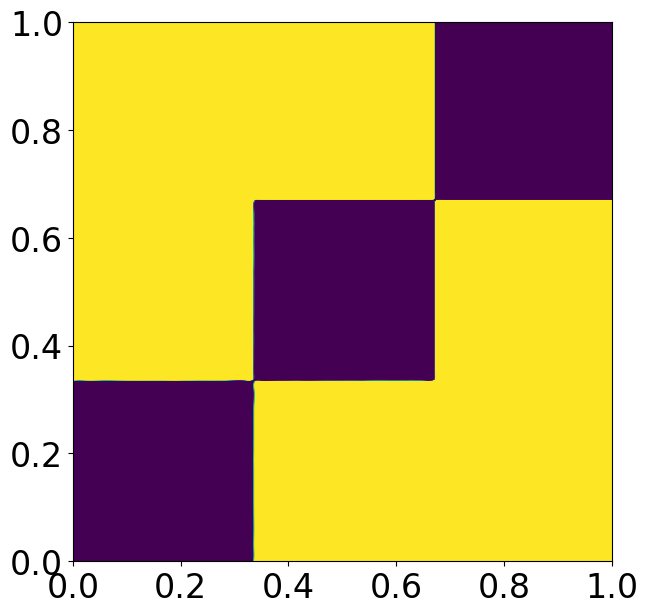
\includegraphics[width=\linewidth]{new_figures/k3_67.png}
      \caption{$p{=}2/3$.}\label{fig:k3-67}
    \end{subfigure}\hfill
    \begin{subfigure}{0.31\linewidth}
      
\includegraphics[width=\linewidth]{new_figures/k3_80.png}
      \caption{$p{=}4/5$.}\label{fig:k3-80}
    \end{subfigure}\\[0.3em]
    \begin{subfigure}{0.31\linewidth}
      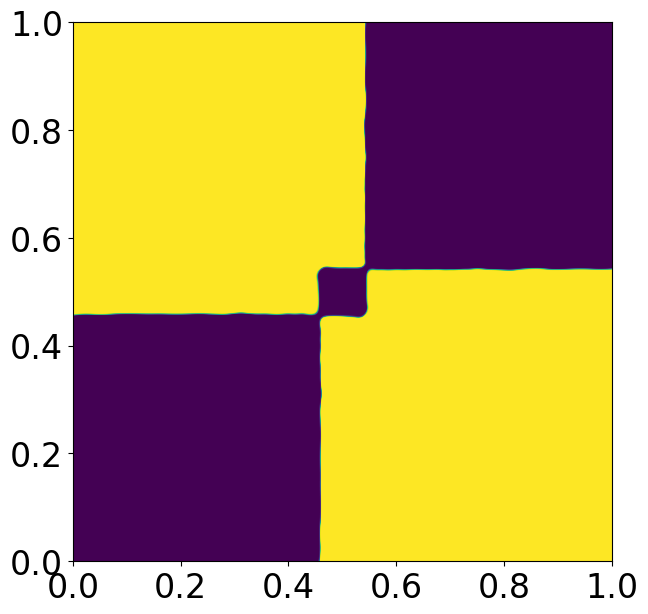
\includegraphics[width=\linewidth]{new_figures/k3_57.png}
      \caption{$p{=}4/7$.}\label{fig:k3-57}
    \end{subfigure}\hfill
    \begin{subfigure}{0.31\linewidth}
      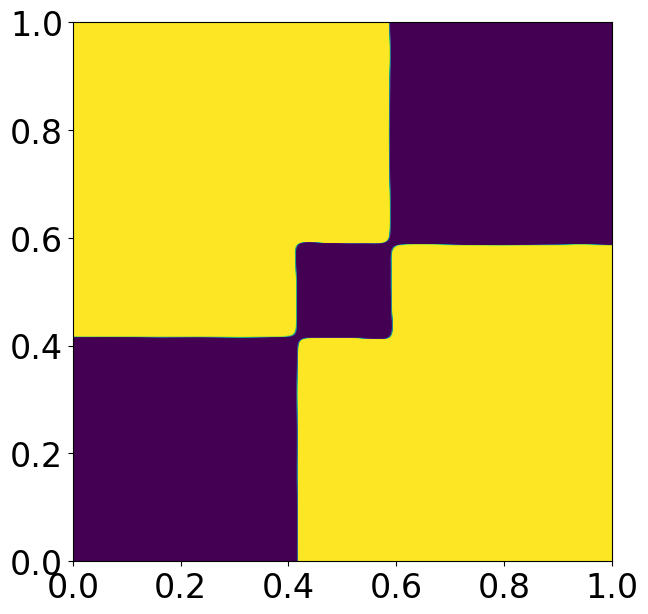
\includegraphics[width=\linewidth]{new_figures/k3_62.png}
      \caption{$p{=}5/8$.}\label{fig:k3-62}
    \end{subfigure}\hfill
    \begin{subfigure}{0.31\linewidth}
      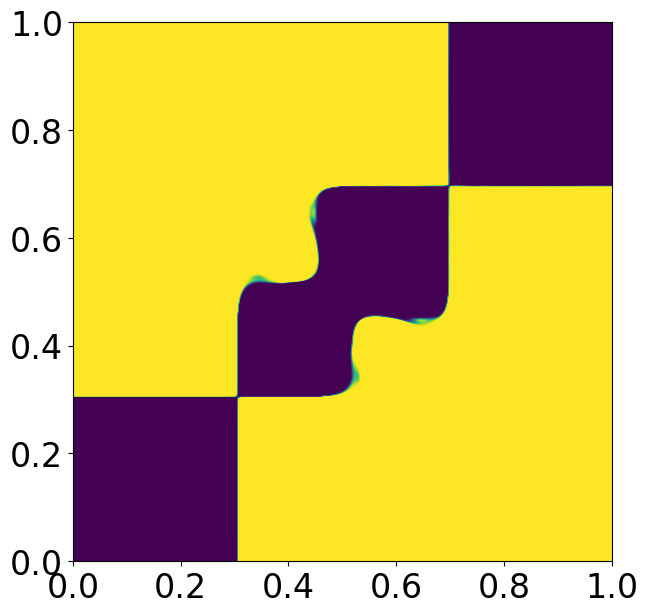
\includegraphics[width=\linewidth]{new_figures/k3_71.png}
      \caption{$p{=}5/7$.}\label{fig:k3-71}
    \end{subfigure}
    \captionof{figure}{Graphons found by our method for $K_3$ density minimisation under $t(K_2, W)=p$.}
    \label{fig:triangledensity-minimisers}
  \end{minipage}
\end{figure}

\begin{figure}[t]
  \centering
  \begin{minipage}{0.55\textwidth}
    \centering
    \captionof{table}{$K_k$ densities in graphons found by our method and the optimal construction for $K_k$ density minimisation under $t(K_2, W) {=} 1 {-} 1/k$. \label{tab:exp2table}}
    {\setlength{\tabcolsep}{4pt}\small
    \begin{tabular}{cll}
       \toprule
       $\mathbf{k}$& \textbf{Optimum} & \textbf{Ours (Estimated)} \\
       \midrule
       $k=4$ & $0.09375$    & $(\mathit{0.09403727}, \mathit{0.09411154})$ \\
       $k=5$ & $0.0384$     & $(\mathit{0.03868024}, \mathit{0.03872081})$ \\
       $k=6$ & $0.01543210$ & $(\mathit{0.01565511}, \mathit{0.01568170})$ \\
       \bottomrule
    \end{tabular}
    }
  \end{minipage}\hfill
  \begin{minipage}{0.40\textwidth}
    \centering
    \begin{subfigure}{0.31\linewidth}
      
\includegraphics[width=\linewidth]{new_figures/k4_75.png}
      \caption{$k{=}4$.}\label{fig:k4-75}
    \end{subfigure}\hfill
    \begin{subfigure}{0.31\linewidth}
      
\includegraphics[width=\linewidth]{new_figures/k5_80.png}
      \caption{$k{=}5$.}\label{fig:k5-80}
    \end{subfigure}\hfill
    \begin{subfigure}{0.31\linewidth}
      
\includegraphics[width=\linewidth]{new_figures/k6_83.png}
      \caption{$k{=}6$.}\label{fig:k6-833}
    \end{subfigure}
    \captionof{figure}{Graphons found by our method for $K_k$ density minimisation under $t(K_2, W) = 1 - 1/k$.}
    \label{fig:clique}
  \end{minipage}
\end{figure}

Computing $\nabla_\theta \widehat{t}_{\mathcal{D}}(H, f_\theta[c_\theta])$ requires only the standard product rule once $\nabla_\theta f_\theta[c_\theta]$ is known; the only non-routine ingredient is the gradient of the solver output $c_\theta$ with respect to $\theta$, which we compute via implicit differentiation.
A direct alternative is to differentiate through an unrolled Newton iteration with autodiff, but this requires storing every intermediate iterate and is substantially more expensive in time and memory; the same trade-off motivates implicit-differentiation methods in deep equilibrium models~\citep{bai2019deep} and neural ODEs~\citep{chen2018neural}. The closed-form gradient is given by:

\begin{lemma}\label{lem:implicitdifferentiation}
For all $\mathbf{x} \in [0,1]^2$,
\begin{align*}
\nabla_\theta\, f_\theta[c_\theta](\mathbf{x})
\,&=\, \frac{\partial f_\theta[c](\mathbf{x})}{\partial \theta}\bigg|_{c = c_\theta}
\,-\, \mathit{sm}'\bigl(h_\theta(\mathbf{x}) + c_\theta\bigr)
\sum_{\mathbf{y} \in \mathcal{E}} w_\theta(\mathbf{y})\, \nabla_\theta h_\theta(\mathbf{y}),
\\
\text{where }
w_\theta(\mathbf{y}) \,&\coloneqq\, \frac{\mathit{sm}'(h_\theta(\mathbf{y}) + c_\theta)}{\sum_{\mathbf{z} \in \mathcal{E}} \mathit{sm}'(h_\theta(\mathbf{z}) + c_\theta)},
\quad
h_\theta(x_1, x_2) \,\coloneqq\, V g_\theta^{(L)}\!\bigl(\min(x_1, x_2), \max(x_1, x_2)\bigr).
\end{align*}
\end{lemma}

For 	\textbf{(P3)}, despite its different mathematical origins in large deviation theory, the same constrained loop applies with two substitutions: for given $0<q<r < 1$, the edge-density solver is replaced by the triangle-density solver targeting $t(K_3, f_\theta[c]) = r^3$, and the objective is replaced by the Monte Carlo estimate of $h_q(f_\theta[c_\theta])=\int_{[0,1]^2} \mathrm{KL}(\mathrm{Bern}(f_\theta[c_\theta](x,y))\,\|\,\mathrm{Bern}(q))dxdy$, obtained by averaging $\mathrm{KL}(\mathrm{Bern}(f_\theta[c_\theta](x,y))\,\|\,\mathrm{Bern}(q))$ over a fresh batch of pairs $(x,y)$. The sigmoid output ensures the KL objective is differentiable in $\theta$, and an analogous implicit-differentiation formula applies to the triangle-density constraint.

\noindent\textit{Unconstrained problems.}
For 	\textbf{(P2)}, with graphs $H_1, H_2$ and positive integers $m_1, m_2$, we minimise $t(H_1, f_\theta[c])^{m_2} - t(H_2, f_\theta[c])^{m_1}$. Using~\eqref{eqn:elimination densityproduct}, we rewrite the objective as $t(H_1^{\oplus m_2}, f_\theta[c]) - t(H_2^{\oplus m_1}, f_\theta[c])$, where $H^{\oplus m}$ is the disjoint union of $m$ copies of $H$, and optimise $(\theta, c)$ by SGD on freshly resampled batches each iteration, applying~\eqref{eqn:estimator} to each term separately.

\begin{figure}[t]
  \centering
  \begin{minipage}{0.40\textwidth}
    \centering
    \captionof{table}{$C_5$ densities in graphons found by our method and the conjectured construction for $C_5$ density minimisation under $t(K_2, W)=p$.\label{tab:c5result}}
    {\setlength{\tabcolsep}{4pt}\small
    \begin{tabular}{cll}
       \toprule
       $\mathbf{p}$ & \textbf{Conjectured} & \textbf{Ours} \\
       \midrule
       $1/2$ & $0$ & $0.00004086$ \\
       $2/3$ & $0.12345679$ & $0.12350364$ ($+0.04\%$) \\
       $4/5$ & $0.3264$ & $0.32644549$ ($+0.01\%$) \\
       $4/7$ & $0.04587149$ & $0.04590020$ ($+0.06\%$) \\
       $5/8$ & $0.08653616$ & $0.08657084$ ($+0.04\%$) \\
       $5/7$ & $0.18200809$ & $0.18206173$ ($+0.03\%$) \\
       \bottomrule
    \end{tabular}
    }
  \end{minipage}\hfill
  \begin{minipage}{0.55\textwidth}
    \centering
    \begin{subfigure}{0.31\linewidth}
      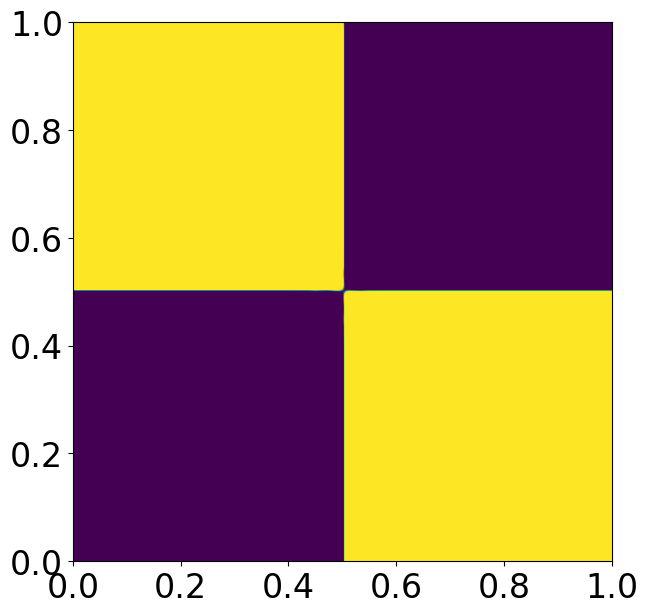
\includegraphics[width=\linewidth]{new_figures/c5_50.png}
      \caption{$p{=}1/2$.}\label{fig:opt-c5-50}
    \end{subfigure}\hfill
    \begin{subfigure}{0.31\linewidth}
      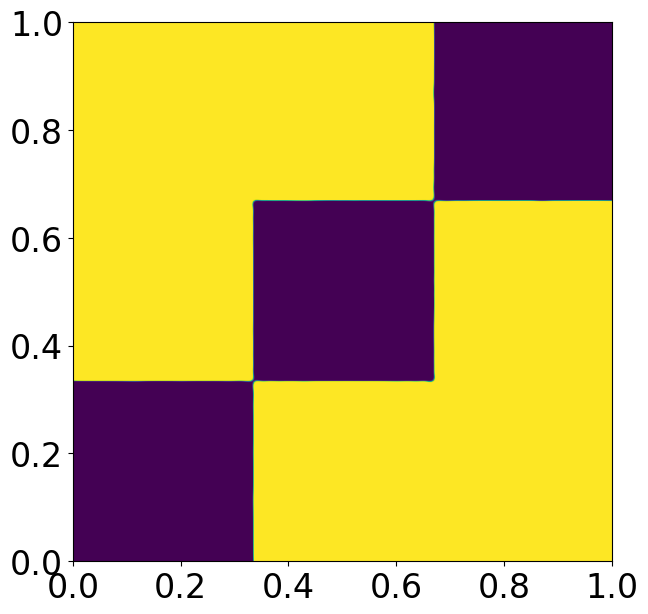
\includegraphics[width=\linewidth]{new_figures/c5_67.png}
      \caption{$p{=}2/3$.}\label{fig:opt-c5-67}
    \end{subfigure}\hfill
    \begin{subfigure}{0.31\linewidth}
      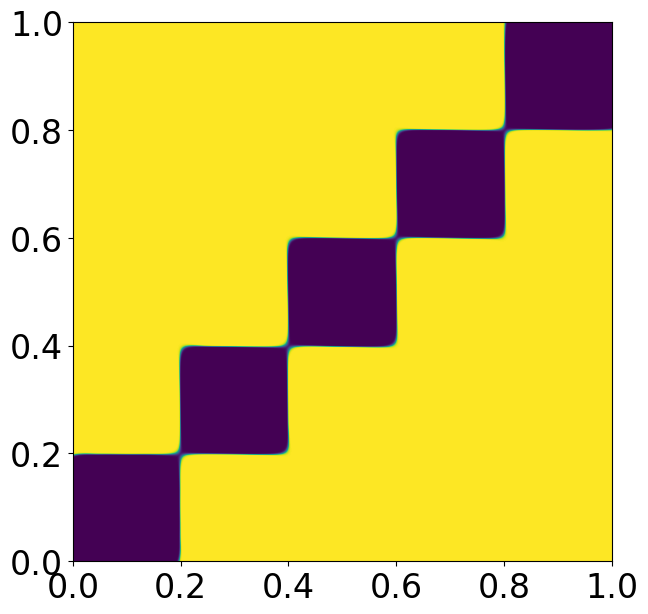
\includegraphics[width=\linewidth]{new_figures/c5_80.png}
      \caption{$p{=}4/5$.}\label{fig:opt-c5-80}
    \end{subfigure}\\[0.3em]
    \begin{subfigure}{0.31\linewidth}
      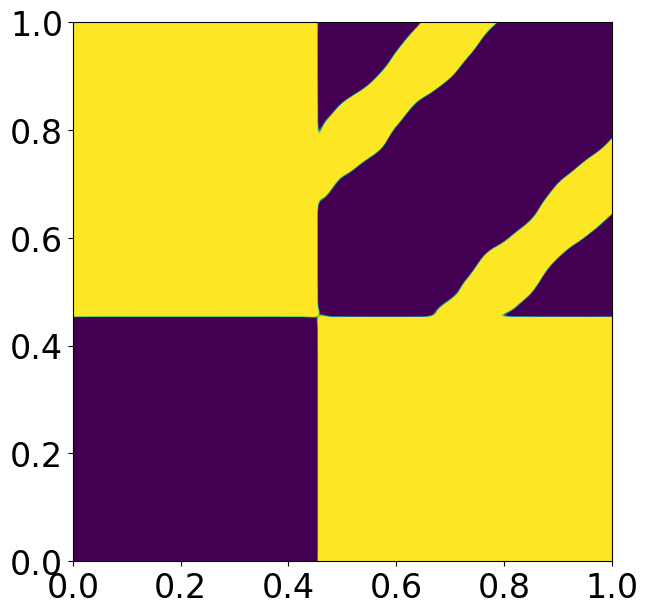
\includegraphics[width=\linewidth]{new_figures/c5_57.png}
      \caption{$p{=}4/7$.}\label{fig:opt-c5-57}
    \end{subfigure}\hfill
    \begin{subfigure}{0.31\linewidth}
      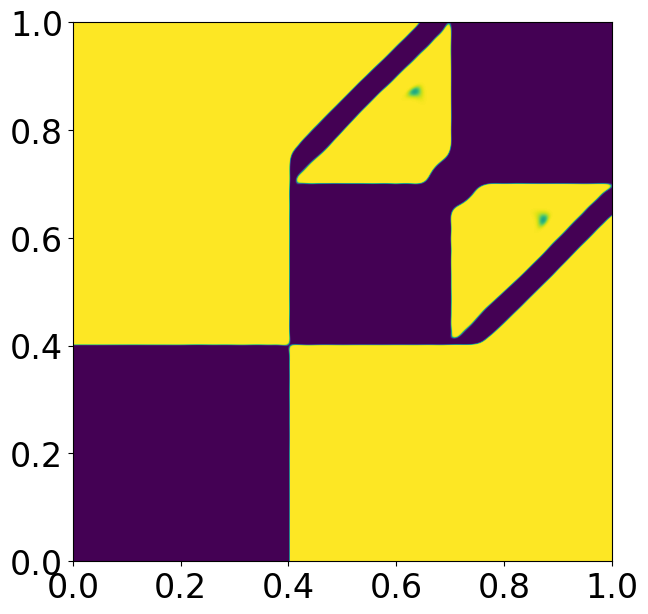
\includegraphics[width=\linewidth]{new_figures/c5_62.png}
      \caption{$p{=}5/8$.}\label{fig:opt-c5-62}
    \end{subfigure}\hfill
    \begin{subfigure}{0.31\linewidth}
      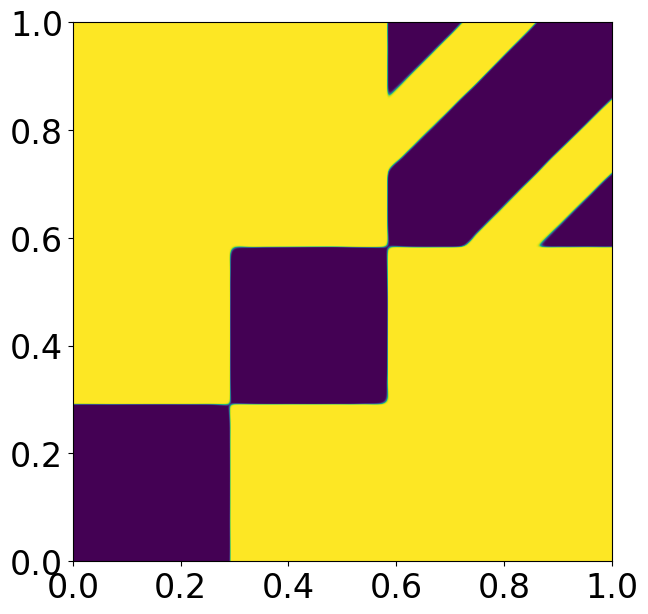
\includegraphics[width=\linewidth]{new_figures/c5_71.png}
      \caption{$p{=}5/7$.}\label{fig:opt-c5-71}
    \end{subfigure}
    \captionof{figure}{Graphons found by our method for $C_5$ density minimisation under $t(K_2, W)=p$.}
    \label{fig:5cycleminimisation}
  \end{minipage}
\end{figure}

\section{Experiment Results} \label{sec:experiments}

We evaluate our framework on instances of 	\textbf{(P1)}, 	\textbf{(P2)}, and 	\textbf{(P3)} drawn from the extremal-graph-theory and large-deviation literatures. The same architecture, solver, and training loop are used throughout; the only changes between problem classes are which constraint, if any, is enforced and how the objective is estimated. The experiments are organised to demonstrate two capabilities: (i) rediscovering classical optima that previously required substantial human effort, and (ii) producing mathematically interesting candidates for open instances. An ablation study at the end isolates the contribution of each architectural component.

We visualise graphons as Viridis heatmaps (blue $\,=\,0$, yellow $\,=\,1$); see \Cref{fig:triangledensity-minimisers}. Reported homomorphism densities are either numerically computed by discretising the learnt graphon into an $M\times M$ weighted adjacency matrix, or estimated using $2^{28}$ samples with a 95\% bootstrap confidence interval (shown in \textit{italic} font) when discretisation is infeasible. Across multiple training runs, we report the lowest-objective run; reported values should be read as best-found candidate upper bounds, and the bootstrap intervals quantify Monte Carlo estimation error rather than variability across runs. See \Cref{sec:experimentdetails} for details.

\paragraph{Constrained homomorphism-density minimisation}
We apply our method to the problem of minimising the homomorphism density of $K_n$ under an edge-density constraint $t(K_2,W)=p$. This is an instance of the first problem in \Cref{eqn:targetproblems}, with $H=K_n$.
For $n=3$ (triangles), this optimisation problem has been studied extensively~\citep{goodman1959on,bollobas1975relations,lovasz1983on,fisher1989lower,razborov2008minimal}, and its full solution was established by~\citet{razborov2008minimal}.
For general $n$, the full solution was obtained more recently by~\citet{reiher2016clique}.


\begin{figure}[t]
  \centering
  \begin{minipage}{0.40\textwidth}
    \centering
    \captionof{table}{$C_7$ densities in graphons found by our method and the conjectured construction for $C_7$ density minimisation under $t(K_2, W)=p$.\label{tab:c7result}}
    {\setlength{\tabcolsep}{4pt}\small
    \begin{tabular}{cll}
       \toprule
       $\mathbf{p}$ & \textbf{Conjectured} & \textbf{Ours} \\
       \midrule
       $1/2$ & $0$ & $0.00001517$ \\
       $2/3$ & $0.05763169$ & $0.05763195$ ($+0.00\%$) \\
       $4/5$ & $0.209664$   & $0.20967621$ ($+0.01\%$) \\
       $4/7$ & $0.01713510$ & $0.01715017$ ($+0.09\%$) \\
       $5/8$ & $0.03610272$ & $0.03611957$ ($+0.05\%$) \\
       $5/7$ & $0.09455118$ & $0.09457182$ ($+0.02\%$) \\
       \bottomrule
    \end{tabular}
    }
  \end{minipage}\hfill
  \begin{minipage}{0.55\textwidth}
    \centering
    \begin{subfigure}{0.31\linewidth}
      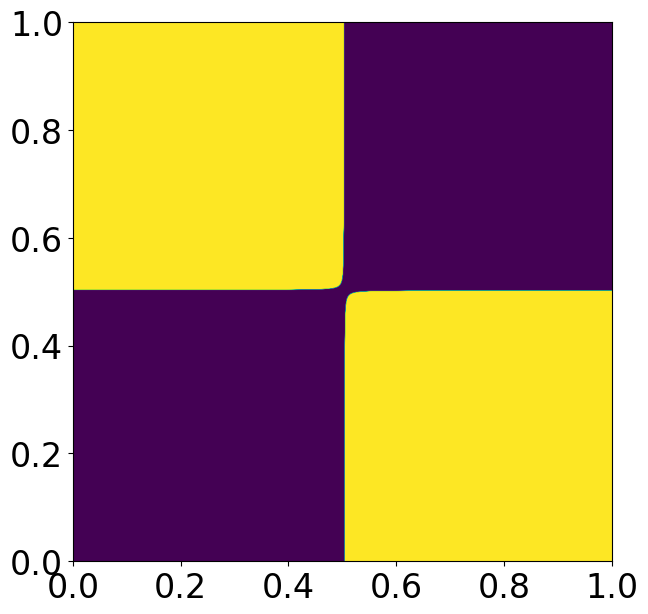
\includegraphics[width=\linewidth]{new_figures/c7_50.png}
      \caption{$p{=}1/2$.}\label{fig:opt-c7-50}
    \end{subfigure}\hfill
    \begin{subfigure}{0.31\linewidth}
      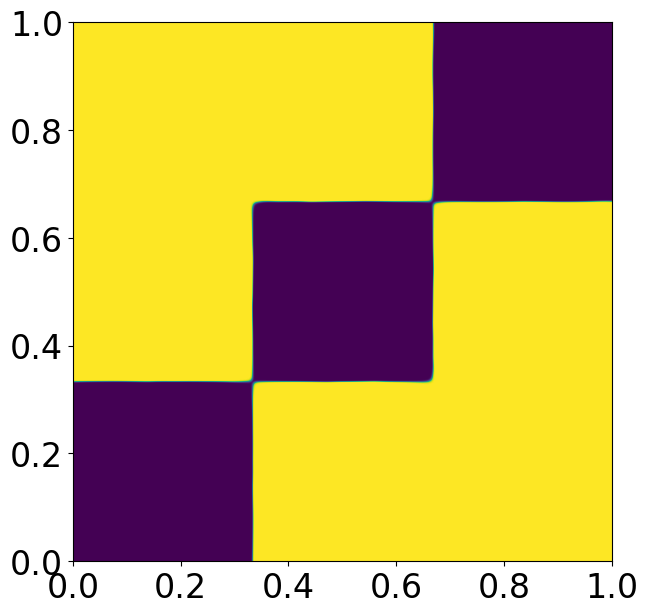
\includegraphics[width=\linewidth]{new_figures/c7_67.png}
      \caption{$p{=}2/3$.}\label{fig:opt-c7-67}
    \end{subfigure}\hfill
    \begin{subfigure}{0.31\linewidth}
      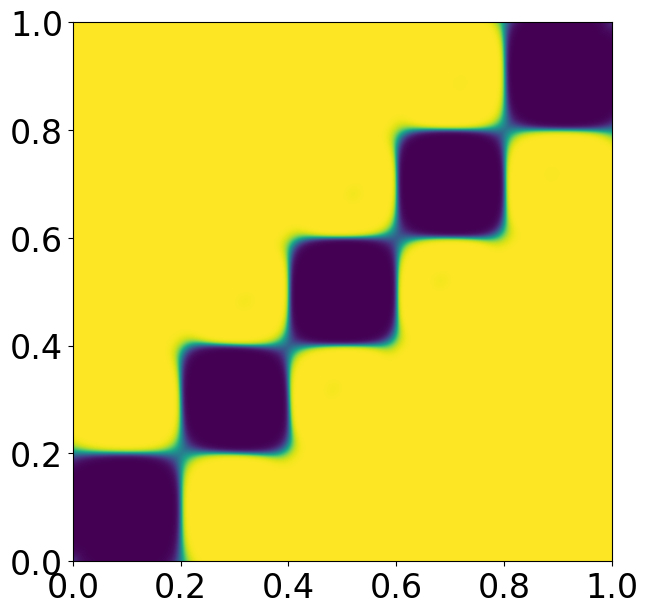
\includegraphics[width=\linewidth]{new_figures/c7_80.png}
      \caption{$p{=}4/5$.}\label{fig:opt-c7-80}
    \end{subfigure}\\[0.3em]
    \begin{subfigure}{0.31\linewidth}
      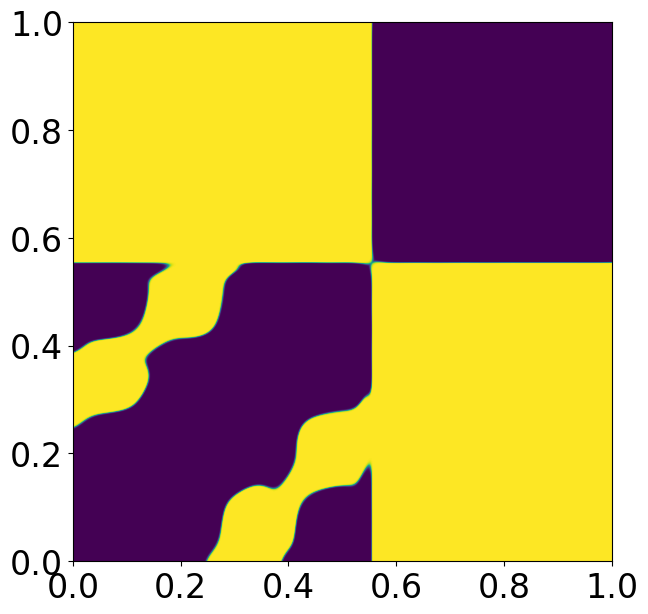
\includegraphics[width=\linewidth]{new_figures/c7_57.png}
      \caption{$p{=}4/7$.}\label{fig:opt-c7-57}
    \end{subfigure}\hfill
    \begin{subfigure}{0.31\linewidth}
      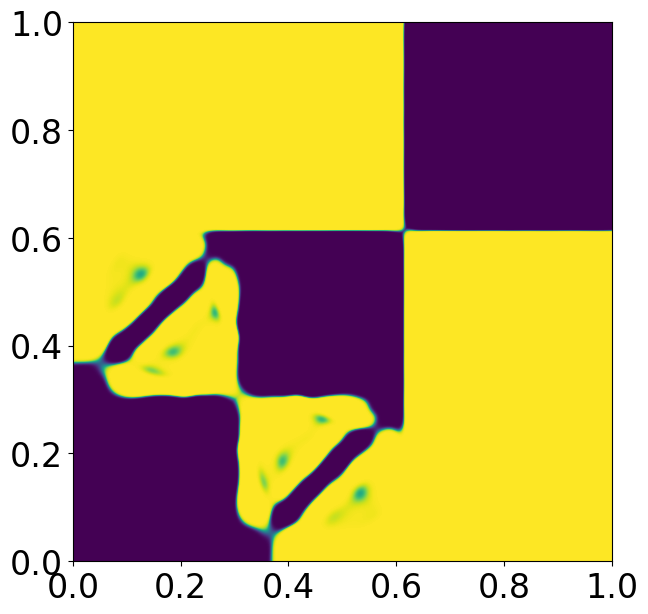
\includegraphics[width=\linewidth]{new_figures/c7_62.png}
      \caption{$p{=}5/8$.}\label{fig:opt-c7-62}
    \end{subfigure}\hfill
    \begin{subfigure}{0.31\linewidth}
      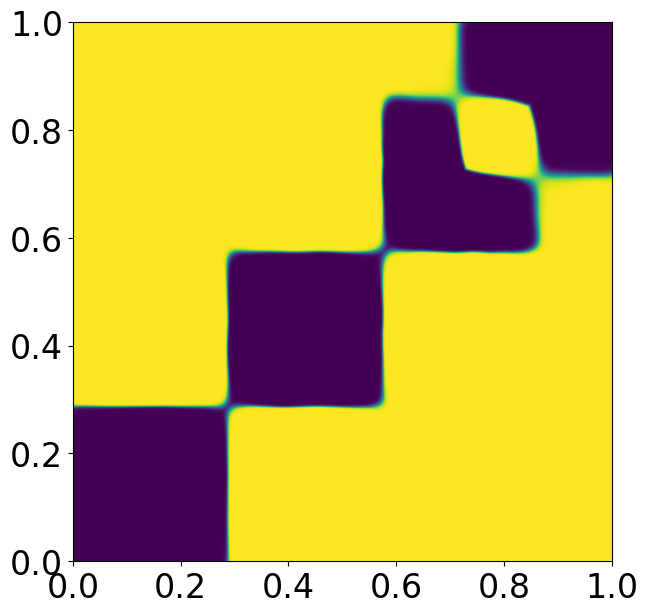
\includegraphics[width=\linewidth]{new_figures/c7_71.png}
      \caption{$p{=}5/7$.}\label{fig:opt-c7-71}
    \end{subfigure}
    \captionof{figure}{Graphons found by our method for $C_7$ density minimisation under $t(K_2, W)=p$.}
    \label{fig:7cycleminimisation}
  \end{minipage}
\end{figure}


We begin with the case $n\,{=}\,3$. When $p \,{=}\, 1 \,{-}\, 1/k$ for some integer $k \ge 2$, the optimal graphon is the complete $k$-partite graphon or any of its measure-preserving permutations.  
For $i \in [k]$, let $X_i = [(i-1)/k, i/k]$. The complete $k$-partite graphon $W_k$ is defined as follows:
$W_k(x_1,x_2) =
1$ if $x_1 \in X_i$ and $x_2 \in X_j$ with $i \neq j$; otherwise,
$W_k(x_1,x_2) = 0$.
For a measure-preserving $\phi$ on $[0,1]$, its permutation is
$W_{k,\phi}(x_1,x_2) = W_k(\phi(x_1), \phi(x_2))$. Every optimum is of this form.
When $1 - 1/k < p < 1 - 1/(k+1)$, the minimisation admits multiple types of optima.  
One example is a variant $W_p$ of $W_{k+1}$, %the $(k+1)$-partite graphon, 
where the first $k$ parts are equal in length but the last part $X_{k+1}$ is shorter.  
Again, its permutations $W_{p,\phi}$ by measure-preserving $\phi$ on $[0,1]$ are also optimal, though %in this regime
the $W_{p,\phi}$ do not exhaust all optima.

We considered $p \in \{1/2, 2/3, 4/5, 4/7, 5/8, 5/7\}$. For the three cases with $p=1-1/k$ ($p\in\{1/2,2/3,4/5\}$), our method produced near-optimal graphons (top row of \Cref{fig:triangledensity-minimisers}) within $0.1\%$ of the theoretical optima, closely matching the complete $k$-partite graphons $W_k$; among the equivalent measure-preserving permutations, our method consistently converged to these simpler representatives.
For $p\in\{4/7,5/8\}$, which satisfy $1-1/k<p<1-1/(k+1)$, the learnt graphons (Fig.~\ref{fig:triangledensity-minimisers}d and \ref{fig:triangledensity-minimisers}e) capture the core structure of the known optimal $W_p$.
For $p=5/7$, the learnt graphon (Fig.~\ref{fig:triangledensity-minimisers}f) does not match $W_p$, but its bipartite middle-block structure matches the characterisation of all optimal graphons in~\citep{pikhurko2017asymptotic}.

\begin{figure}[t]
  \centering
  \begin{minipage}{0.42\textwidth}
    \centering
    \captionof{table}{$H_6$ densities in graphons found by our method, the $k$-partite construction, and the constant graphon, for $H_6$ density minimisation under $t(K_2, W){=}p$.\label{tab:noveloptimum}}
    {\setlength{\tabcolsep}{4pt}\small
    \begin{tabular}{clll}
      \toprule
      $\mathbf{p}$ & \textbf{Ours} & \textbf{$k$-partite} & \textbf{Constant} \\
      \midrule
      $2/3$ & $0.02476414$ & $0.03292181$ & $0.02601229$ \\
      $3/4$ & $0.07218717$ & $0.07617188$ & $0.07508469$ \\
      $4/5$ & $0.12985603$ & $0.13056$    & $0.13421773$ \\
      \bottomrule
    \end{tabular}
    }
  \end{minipage}\hfill
  \begin{minipage}{0.55\textwidth}
    \centering
    \begin{subfigure}{0.23\linewidth}
      \centering
      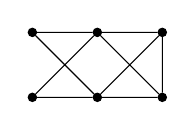
\begin{tikzpicture}[scale=0.55]
        \node[circle, draw, fill=black, minimum size=3pt, inner sep=0pt] (v1) at (-1.5, 1.5) {};
        \node[circle, draw, fill=black, minimum size=3pt, inner sep=0pt] (v2) at (-1.5, 0) {};
        \node[circle, draw, fill=black, minimum size=3pt, inner sep=0pt] (v3) at (0, 1.5) {};
        \node[circle, draw, fill=black, minimum size=3pt, inner sep=0pt] (v4) at (0, 0) {};
        \node[circle, draw, fill=black, minimum size=3pt, inner sep=0pt] (v5) at (1.5, 1.5) {};
        \node[circle, draw, fill=black, minimum size=3pt, inner sep=0pt] (v6) at (1.5, 0) {};
        \draw (v5) -- (v4) -- (v1) -- (v3) -- (v5) -- (v6) -- (v3) -- (v2) -- (v4) -- (v6);
      \end{tikzpicture}
      \caption{$H_6$.}
      \label{fig:graph-222}
    \end{subfigure}\hfill
    \begin{subfigure}{0.23\linewidth}
      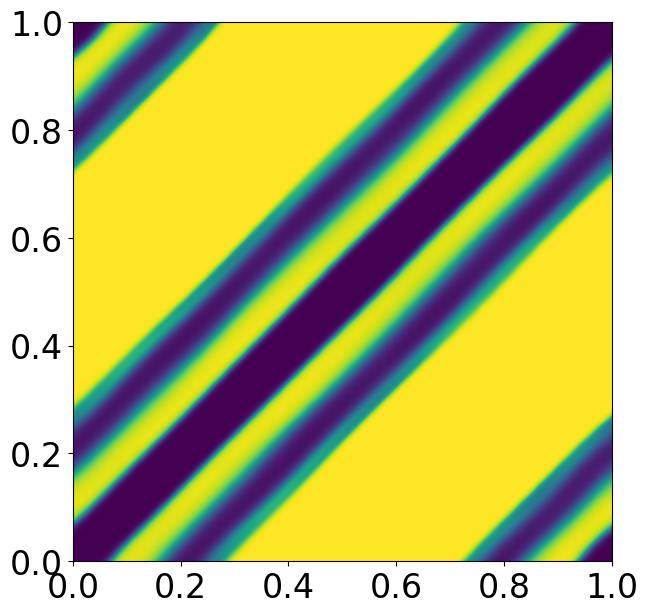
\includegraphics[width=\linewidth]{new_figures/222_67.png}
      \caption{$p{=}2/3$.}
      \label{fig:opt-222-67}
    \end{subfigure}\hfill
    \begin{subfigure}{0.23\linewidth}
      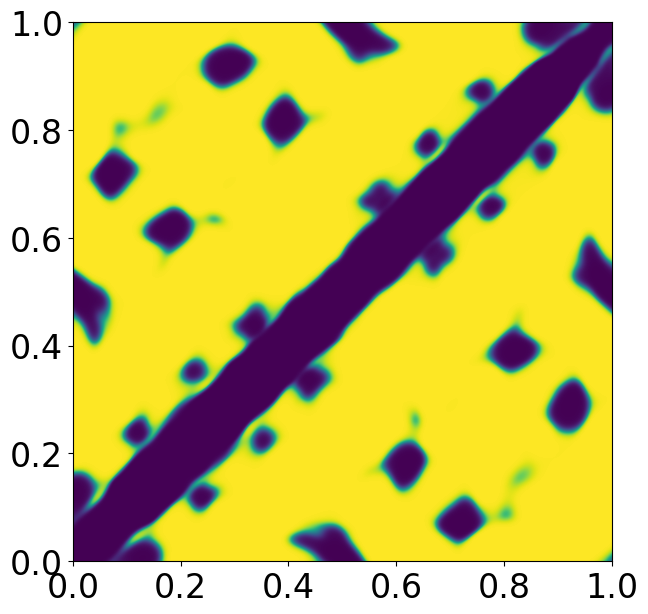
\includegraphics[width=\linewidth]{new_figures/222_75.png}
      \caption{$p{=}3/4$.}
      \label{fig:opt-222-75}
    \end{subfigure}\hfill
    \begin{subfigure}{0.23\linewidth}
      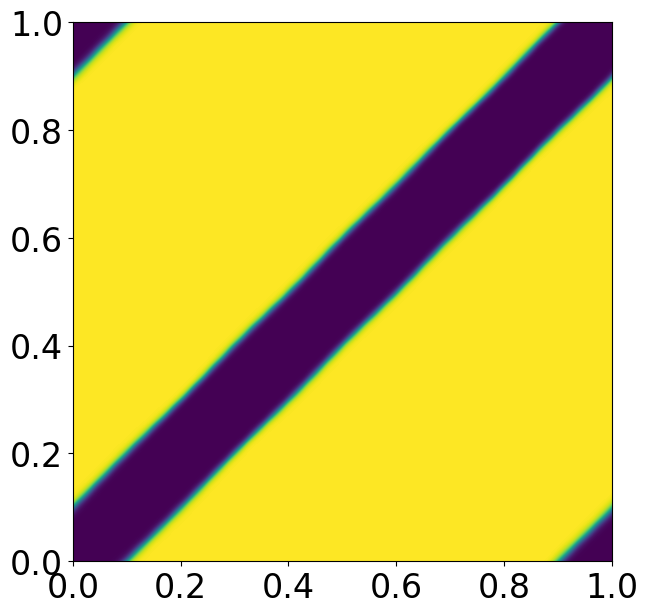
\includegraphics[width=\linewidth]{new_figures/222_80.png}
      \caption{$p{=}4/5$.}
      \label{fig:opt-222-80}
    \end{subfigure}
    \captionof{figure}{The graph $H_6$ (six vertices, nine edges) and graphons found by our method for $H_6$ density minimisation under $t(K_2, W) = p$.}
    \label{fig:noveloptimum}
  \end{minipage}
\end{figure}

For $K_k$ with $k>3$, we ran $\min_W t(K_k, W)$ s.t.\ $t(K_2, W){=}1{-}1/k$ for $k\in\{4,5,6\}$. Even though the larger motif size increases the variance of our estimator and the optimal graphon involves more blocks, our method recovers the complete $k$-partite structure (\Cref{fig:clique}).

\begin{figure}[t]
  \centering
  \begin{minipage}{0.45\textwidth}
    \centering
    \captionof{table}{Difference of normalised homomorphism densities of $K_r, K_s$ in graphons found by our method. Negative estimates indicate violations by the learnt graphon.\label{tab:cliquedensitycomparison}}
    {\small
    \begin{tabular}{lc}
       \toprule
       & $t(K_r,W)^{\binom{s}{2}} - t(K_s,W)^{\binom{r}{2}}$ \\
       \midrule
       $r=3, s=4$ & $\mathit{-0.05948110}$ \\
       $r=3, s=5$ & $\mathit{-0.24935071}$ \\
       $r=4, s=5$ & $\mathit{-0.07295104}$ \\
       \bottomrule
    \end{tabular}
    }
  \end{minipage}\hfill
  \begin{minipage}{0.50\textwidth}
    \centering
    \begin{subfigure}{0.31\linewidth}
      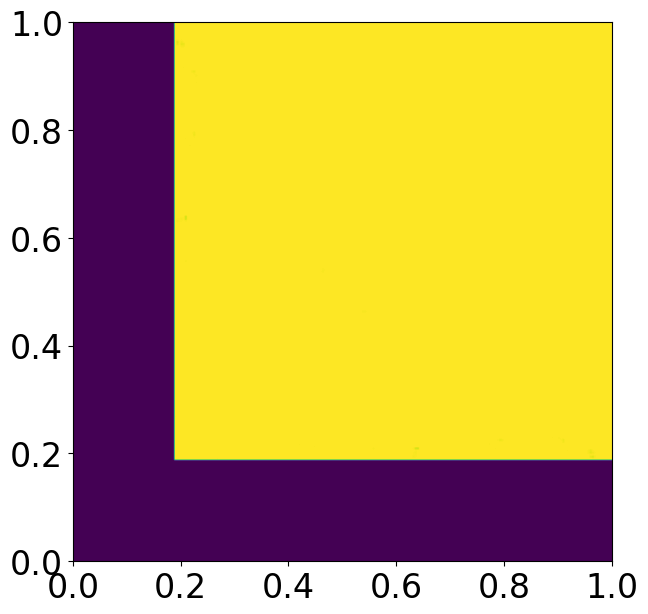
\includegraphics[width=\linewidth]{figures/k3_k4.png}
      \caption{$(r,s){=}(3,4)$.}\label{fig:k3_k4}
    \end{subfigure}\hfill
    \begin{subfigure}{0.31\linewidth}
      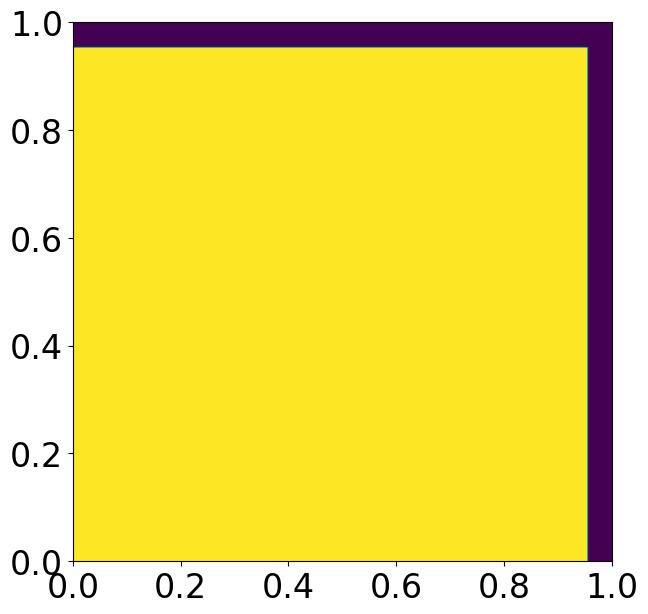
\includegraphics[width=\linewidth]{figures/k3_k5.png}
      \caption{$(r,s){=}(3,5)$.}\label{fig:k3_k5}
    \end{subfigure}\hfill
    \begin{subfigure}{0.31\linewidth}
      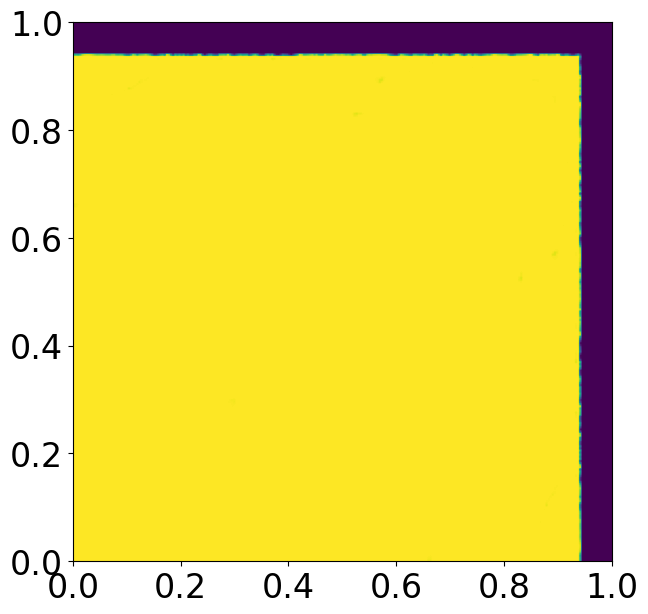
\includegraphics[width=\linewidth]{figures/k4_k5.png}
      \caption{$(r,s){=}(4,5)$.}\label{fig:k4_k5}
    \end{subfigure}
    \captionof{figure}{Graphons found by our method for the minimisation of $t(K_r,W)^{\binom{s}{2}} - t(K_s,W)^{\binom{r}{2}}$.}
    \label{fig:cliqueinequality}
  \end{minipage}
\end{figure}

\noindent{\it Unresolved Problems: $C_5$ and $C_7$.}
We next apply our method to two graphon optimisation problems that, to the best of our knowledge, remain open in the tested regimes: minimising the homomorphism densities of $C_5$ and $C_7$, each under a fixed edge density~$p$. In \Cref{sec:addexperiments}, we also report results for the Petersen graph, for which no prior optima or conjectured optima are known to us.

For $C_5$, \citet{bennet2020minimizing} characterised the minimisers when $p=1-1/k$ and conjectured them for other $p$. We applied our method for $p\in\{1/2, 2/3, 4/5, 4/7, 5/8, 5/7\}$ (\Cref{fig:5cycleminimisation}); the resulting values agree with the benchmark optima within $0.1\%$ (\Cref{tab:c5result}). When $p=1-1/k$ the learnt graphon recovers the complete $k$-partite structure (top row); for other $p$ it exhibits pronounced diagonal (banded) structure (bottom row), suggesting a qualitatively different extremal configuration away from the rational breakpoints.

For $C_7$, no prior results are known to us. Motivated by the $C_5$ results of \citet{bennet2020minimizing}, we propose a conjecture for the structure and optimum value of $C_7$-minimising graphons under a fixed edge density; see \Cref{sec:oddcycleconjecture}. Empirically, our learnt graphons match the conjectured optima within $0.1\%$ across all tested $p$ (\Cref{tab:c7result}). For $p\in\{1/2,2/3,4/5\}$ ($p=1-1/k$), they recover the complete $k$-partite structure (top row of \Cref{fig:7cycleminimisation}); for $p\in\{4/7,5/8\}$ they show diagonal patterns similar to $C_5$, suggesting that this is a common feature of odd-cycle minimisation; for $p=5/7$ the structure is qualitatively different, with block-like rather than diagonal patterns (bottom-right of \Cref{fig:7cycleminimisation}).

\noindent{\it Exhaustive study over small graphs.}
We now describe a systematic study enabled by our method.
We applied our method to the first problem in \Cref{eqn:targetproblems} for non-bipartite graphs $H$ with $v(H) \le 6$ and $e(H) \le 9$, and with no isolated vertices, for a total of 175 graphs.
For each $H$, we trained our network to minimise $t(H,W)$ subject to $t(K_2,W)=p$, for
$p \in \{\frac{k-2}{k-1},\ \frac{3k-5}{3k-2},\ \frac{2k-3}{2k-1},\ \frac{3k-4}{3k-1},\ \frac{k-1}{k}\}$,
% \[
% p \in \left\{\frac{k-2}{k-1},\ \frac{3k-5}{3k-2},\ \frac{2k-3}{2k-1},\ \frac{3k-4}{3k-1},\ \frac{k-1}{k}\right\},
% \]
where $k$ is the chromatic number of $H$.
These values of $p$ are chosen to probe the structure of the curve
$x \mapsto \min_{t(K_2,W)=x} t(H,W)$:
the first and last values correspond to breakpoints of piecewise-defined curves established for several families of graphs~\citep{razborov2008minimal,reiher2016clique,bennet2020minimizing}, while the remaining values lie in the interior of the corresponding segments.
We also implemented an automated tool for computing lower bounds on the minimum $H$-density using flag algebras~\citep{razborov2007flag}, which we used in our experiments.

Across 76.5\% of the $(H,p)$ instances, our method produced a graphon whose $H$-density closely matches the corresponding flag-algebra lower bound (within $1\%$ relative error, or $10^{-6}$ absolute when the bound is near zero), suggesting that the solutions are optimal or near-optimal. Of the rest, 11.8\% were clearly suboptimal or failed to train, while for the remaining 11.7\% the learnt graphons appear optimal but our flag-algebra bounds were not tight.

We analysed the curve $x \mapsto \min_{t(K_2,W)=x} t(H,W)$ for each $H$, by interpolation, and examined whether it appears piecewise concave (as for cliques~\citep{reiher2016clique}) or convex (as conjectured for odd cycles~\citep{bennet2020minimizing}). Apparent piecewise concavity is associated with graphs close to complete graphs (i.e., complete after removing $1$ or $2$ edges and isolated vertices); the other graphs gave apparently convex curves.

Our experiments also suggest a novel family of extremal graphon structures. When $p \,{=}\, 1 \,{-}\, 1/k$ for an integer $k \,{\ge}\, 2$, the minimisers in \Cref{fig:triangledensity-minimisers,fig:5cycleminimisation,fig:7cycleminimisation} are uniquely characterised (up to measure-preserving transformations) as complete $k$-partite graphons. This is not universal: for the graph $H_6$ in Fig.~\ref{fig:noveloptimum}a at the same $p$, our method finds a candidate minimiser that is neither complete $k$-partite nor constant (\Cref{fig:noveloptimum}); the learnt graphons exhibit a geometric pattern in which edge probabilities appear to depend on the circular distance when $[0,1]$ is interpreted as a circle.

\paragraph{Normalised inequalities between densities}
For 	\textbf{(P2)}, we searched for graphons violating proposed inequalities $t(H_1,W)^{m_2} \geq t(H_2,W)^{m_1}$. As an illustrative task, for each $r,s \in \{3,4,5\}$ with $r < s$, we considered the edge-normalised inequality $t(K_r, W)^{\binom{s}{2}} \ge t(K_s, W)^{\binom{r}{2}}$. For all tested pairs, our method found graphons (\Cref{fig:cliqueinequality}) with negative objective, strongly suggesting failure of the inequalities; see \Cref{tab:cliquedensitycomparison}.

\paragraph{Variational problem from large deviation theory}
We finally apply our framework to 	\textbf{(P3)}, the upper-tail variational problem of \citet{chatterjee2011large}. The architecture, optimiser, and training loop carry over from 	\textbf{(P1)}; only the edge-density solver is replaced by the triangle-density solver targeting $t(K_3, W) = r^3$ and the objective is the Monte Carlo estimate of $h_q$. We test $(q,r) \in \{0.05, 0.1\} \times \{0.4, 0.5, 0.6\}$, a small-$q$, moderate-$r$ regime in which the structure of optimisers is, to our knowledge, not fully understood. As a reference we use the one-clique-on-uniform construction $W_{\mathrm{LZ}}$ proposed by \citet{lubetzky2015replica}; \Cref{tab:largedeviation} compares $h_q(W_{\mathrm{LZ}})$ to $h_q$ at our learnt graphon. \TODO{Fill in: (i) qualitative structure of the learnt graphons (e.g., whether a consistent two-block / SBM pattern emerges across $(q,r)$); (ii) quantitative comparison summary; (iii) the resulting structural conjecture, placed in the context of the replica-symmetry boundary of \citet{lubetzky2015replica}.}

\begin{table}[t]
  \centering
  \captionof{table}{Relative-entropy $h_q(W)$ at our learnt graphon ($W_{\mathrm{ours}}$) and at the one-clique-on-uniform construction $W_{\mathrm{LZ}}$ of \citet{lubetzky2015replica}, for 	\textbf{(P3)} on $(q,r) \in \{0.05, 0.1\} \times \{0.4, 0.5, 0.6\}$. Lower is better.\label{tab:largedeviation}}
  {\small
  \begin{tabular}{lcccccc}
    \toprule
    & \multicolumn{3}{c}{$q=0.05$} & \multicolumn{3}{c}{$q=0.10$} \\
    \cmidrule(lr){2-4}\cmidrule(lr){5-7}
    $r$ & $0.4$ & $0.5$ & $0.6$ & $0.4$ & $0.5$ & $0.6$ \\
    \midrule
    $h_q(W_{\mathrm{LZ}})$    & $0.556049$ & $0.830366$ & $1.144945$ & $0.311239$ & $0.510825$ & $0.750684$ \\
    $h_q(W_{\mathrm{ours}})$  & $0.460461$ & $0.725292$ & $1.051539$ & $0.308220$ & $0.506100$ & $0.747289$ \\
    \bottomrule
  \end{tabular}
  }
\end{table}

\paragraph{Ablation study, baselines, and multi-task variant}
An ablation study on triangle-density minimisation under $t(K_2, W) = 7/9$ confirms that each component of our architecture matters: removing the multi-scale sinusoidal encoding, the constraint solver, or the cosine-annealing schedule consistently degrades the recovered structure or its accuracy. On the same task, four non-neural baselines tailored to step graphons (a fixed-block SBM with $256$ blocks; SBMs with trainable block sizes; a decision tree; a tree ensemble) all yielded qualitatively poorer solutions than even the ablated variants. A preliminary FiLM-conditioned multi-task variant jointly trained over $p \in [1/2, 2/3]$ for $H = K_3$ further shows that shared training across related tasks is feasible. Full details are deferred to \Cref{sec:ablation}.


% Broader impacts are addressed in the NeurIPS Paper Checklist; in short,
% this work presents a tool for accelerating mathematical discovery in
% extremal graph theory, with no major foreseeable negative societal impacts.

\bibliography{references}
\bibliographystyle{plainnat}

\appendix

\newpage

\allowdisplaybreaks[0]

\section{Related Work}

Razborov's \emph{flag algebra} framework~\citep{razborov2007flag} enables the proofs of inequalities between graph homomorphism densities by means of sums of squares (ultimately, applications of the Cauchy--Schwarz inequality) in an algebra of graphs, where each finite graph can be interpreted as a functional on the space of graphons. This viewpoint enables the automation of Cauchy--Schwarz-style arguments via semidefinite programming (SDP), and has been implemented in the package {\sc Flagmatic}~\citep{falgas2013applications}.
Flag algebras and Flagmatic have resolved many open problems in extremal combinatorics over the past decade (for a survey, see~\citet{razborov2013survey}), but their computational cost can be prohibitive\footnote{For example, to derive a nontrivial inequality for a graph $G$, {\sc Flagmatic} typically enumerates all graphs $H$ with $v(H) \geq v(G)+1$ and solves an SDP over vectors indexed by such graphs. Graphs $H$ with more than eight vertices are currently unsupported due to computational complexity.}.
This limits applicability to some instances we consider, such as problems involving the Petersen graph.
We view our method as \emph{complementary} to flag algebras rather than a replacement: flag algebras provide rigorous \emph{lower} bounds together with certificates, whereas our method searches directly for candidate graphons and yields candidate \emph{upper} bounds and concrete candidate minimisers. When an upper bound from our method nearly matches a rigorous lower bound, this gives strong evidence for the correct optimum and produces a graphon whose structure can be inspected and turned into mathematical conjectures (as in our exhaustive sweep in \Cref{sec:experiments}).

For fixed values of $n$ (i.e., without taking the limit in \Cref{eqn:extremalproblem:generalisedTuran,eqn:extremalproblem:dominationExponent} or related formulations), one may instead attempt to solve the discrete optimisation problem directly. A classical approach is local (e.g., Tabu) search, which remains useful in combination with reinforcement learning; see, e.g.,~\citet{parczyk2024new,mehrabian2024finding}.
As a direct reinforcement-learning approach, \citet{mehrabian2024finding} used {\sc AlphaZero} to find the maximum number of edges in an $n$-vertex graph with no copies of $K_3$ and $C_4$.
Recently, the so-called \emph{deep cross entropy method} built upon reinforcement learning was used by~\citet{adam2021constructions} for analysing discrete problems in combinatorics. It iteratively trains a neural network to learn a policy that promotes the generation of high quality examples, which succeeded in disproving two conjectures regarding the eigenvalue of the adjacency matrix and matching number or proximity.
For discrete objectives, these approaches can be more versatile than our method because they can optimise non-differentiable quantities (e.g., the matching number). In contrast, they operate at a fixed graph size, whereas our method targets asymptotic problems in the dense-graph limit.
Finally, {\sc PatternBoost}~\citep{charton2024patternboost} takes a hybrid approach that combines local search with reinforcement learning; one illustrative example is generating lower-bound examples related to Mantel's theorem by solving finite-$n$ instances of \Cref{eqn:extremalproblem:generalisedTuran} for $H=K_3$ (for small $n$) up to edge density $p \le 1/2$.
Because many combinatorial objects are highly symmetric, solutions produced by such discrete approaches can be difficult to interpret or distil into human-understandable structure. 
In contrast, as demonstrated by visualisations of learned graphons, our method often captures structure that is amenable to inspection and interpretation.

From the perspective of implicit neural representations, the work most closely related to ours is \citet{mundinger2025neural}, which applies implicit neural representations to the Hadwiger--Nelson problem: colouring the plane $\mathbb{R}^2$ with the minimum number of colours such that no two points at unit distance share a colour. Analogously to our approach, they represent a colouring by a neural network and recover a 6-colouring by minimising a monochromatic edge-density objective. With human post-processing, they construct two new 6-colourings that expand the known range of realisable distances from $[0.415, 0.447]$ to $[0.354, 0.657]$. In contrast, we focus on asymptotic extremal problems in graph theory that can be phrased as constrained optimisation over graphons. Moreover, our approach integrates problem structure into the learning procedure, including an architectural bias toward discontinuous, step-like solutions, explicit constraint enforcement via an embedded solver, and variance reduction in homomorphism density estimation, with the aim of supporting systematic conjecture generation and exploration across diverse extremal problems in graph theory.

\section{Unbiasedness of Our Density Estimator and Proof of the Implicit-Differentiation Lemma}

\begin{lemma} \label{lem:unbiased}
The estimator in~\Cref{eqn:estimator} is unbiased, i.e., $\mathbb{E}[\widehat{t}(H,f_\theta[c])] = t(H,f_\theta[c])$.
\end{lemma}
\begin{proof}[Proof]
We compute the claimed equality as follows:
\begin{align*}
\mathbb{E}\left[\widehat{t}(H, f_\theta{[c]})\right] 
& {} = 
\mathbb{E}\left[\frac{1}{N|\mathcal{S}|} \sum_{k \in [N], \pi \in \mathcal{S}} \left(\prod_{\{i, j\} \in E(H)} f_\theta[c]\Big(x_{\pi(i)}^{(k)}, x_{\pi(j)}^{(k)}\Big)\right)\right]
\\
& {} = 
\frac{1}{N|\mathcal{S}|} \sum_{k \in [N], \pi \in \mathcal{S}} 
\mathbb{E}\left[\prod_{\{i, j\} \in E(H)} f_\theta[c]\Big(x_{\pi(i)}^{(k)}, x_{\pi(j)}^{(k)}\Big)\right]
\\
& {} = 
\frac{1}{N|\mathcal{S}|} \sum_{k \in [N], \pi \in \mathcal{S}} 
\mathbb{E}_{x_1,\ldots,x_{v(H)} \stackrel{\mathrm{iid}}{\sim}\mathrm{Unif}[0,1]}\left[\prod_{\{i, j\} \in E(H)} f_\theta[c](x_i, x_j)\right]
\\
& {} = 
\frac{1}{N{|\mathcal{S}|}} 
\sum_{k \in [N], \pi \in \mathcal{S}} t(H,f_\theta{[c]}) = t(H,f_\theta{[c]}).
\end{align*}
\end{proof}

\begin{proof}[Proof of Lemma~\ref{lem:implicitdifferentiation}]
Let $\mathbf{x} \in [0,1]^2$. Note that
\begin{align*}
    \nabla_\theta\;f_\theta[c_\theta](\mathbf{x}) 
    & = \frac{\partial f_\theta[c](\mathbf{x})}{\partial\theta}\Big|_{c = c_\theta} 
        + \frac{\partial f_\theta[c](\mathbf{x})}{\partial c}\Big|_{c = c_\theta} \nabla_\theta c_\theta
    \\
    & = \frac{\partial f_\theta[c](\mathbf{x})}{\partial\theta}\Big|_{c = c_\theta} 
        + \mathit{sm}'(h_\theta(\mathbf{x}) + c_\theta) \nabla_\theta c_\theta
\end{align*}
Thus, it suffices to show that 
\[
\nabla_\theta c_\theta = 
 {-}  \sum_{\mathbf{y} \in \mathcal{E}}\frac{\mathit{sm}'(h_\theta(\mathbf{y}) + c_\theta)}{\sum_{\mathbf{z} \in \mathcal{E}} \mathit{sm}'(h_\theta(\mathbf{z}) + c_\theta)} \nabla_\theta\, h_\theta(\mathbf{y}).
\]
We prove the above equality by applying implicit differentiation to the following equation about $c_\theta$, which holds by the choice of $c_\theta$:
\[
\frac{1}{|\mathcal{E}|} \sum_{\mathbf{y} \in \mathcal{E}} f_{\theta}[c_\theta](\mathbf{y}) = p.
\]
First, we multiply both sides of the equation by $|\mathcal{E}|$, and differentiate them with respect to $\theta$:
\[ 
\left(\sum_{\mathbf{y} \in \mathcal{E}} \frac{\partial f_{\theta}[c](\mathbf{y})}{\partial \theta}\Big|_{c = c_\theta}\right) 
+ 
\left(\sum_{\mathbf{z} \in \mathcal{E}} \frac{\partial f_{\theta}[c](\mathbf{z})}{\partial c}\Big|_{c = c_\theta} \nabla_\theta c_\theta\right) 
= 0
\]
Thus, 
\begin{align*}
    \nabla_\theta c_\theta 
    & {} = {-} \left(\sum_{\mathbf{y} \in \mathcal{E}} \frac{\partial f_{\theta}[c](\mathbf{y})}{\partial \theta}\Big|_{c = c_\theta}\right) \Bigg/  \left(\sum_{\mathbf{z} \in \mathcal{E}} \frac{\partial f_{\theta}[c](\mathbf{z})}{\partial c}\Big|_{c = c_\theta}\right)
    \\
    & =  {-} \sum_{\mathbf{y} \in \mathcal{E}} \frac{\mathit{sm}'(h_\theta(\mathbf{y}) + c_\theta)}{\sum_{\mathbf{z} \in \mathcal{E}} \mathit{sm}'(h_\theta(\mathbf{z}) + c_\theta)} \nabla_\theta\, h_\theta(\mathbf{y}),
\end{align*}  
as desired.
\end{proof}

\section{Details of Experiments} \label{sec:experimentdetails}

All experiments were conducted on a single NVIDIA RTX A5000 GPU.
The execution time depends on the size of the graph, from 30 minutes for a triangle to a few hours for the Petersen graph.

In all experiments, we used a network of width $d=256$ and depth $L=6$, which was sufficient to represent sharp boundaries and structural properties.
The activation function $\phi$ was either $\sin$ or the GELU nonlinearity; we did not observe a consistent advantage of one over the other.
For the reported main experiments we used the increasing input-encoding scale $s(\ell)=\ell$; the alternative schedule $s(\ell)=2^{\ell-1}$ was used only in pilot runs. The constant-scale schedules in the ablation study are described in \Cref{sec:ablation}.

The set $\mathcal{S}$ in Equation~\Cref{eqn:estimator} was chosen according to the graph. For example, for complete graphs we used $\mathcal{S}=\{\mathrm{id}\}$, since any permutation yields the same summand.
For cycles, we used a set of representatives for the cosets $S_{V(C_k)} / \text{Aut}(C_k)$, where $\text{Aut}(C_k)$ is the automorphism group of $C_k$, which gives $|\mathcal{S}| = (k-1)! / 2$.
For the other graphs, we used the set $\mathcal{S}=\{\pi^k : k \in \mathbb{N}\}$ generated by some permutation $\pi \in S_{V(G)}$, where $\pi$ is chosen so that the set
\[
  \{\{\pi^k(v), \pi^k(w)\} : \{v, w\} \in E(G) \text{ and } k \in \mathbb{N}\}
\]
equals the set of all unordered pairs of distinct vertices $\{\{v, w\} : v, w \in V(G) \text{ and } v \neq w\}$.

For training, we used the largest number of samples that fit in GPU memory, ranging from $2^{12}$ to $2^{16}$.
For large graphs such as the Petersen graph, we repeated multiple forward passes to accumulate gradients, yielding an effective sample size of $2^{16}$.
With caching of pairwise network evaluations, the dominant per-iteration cost scales approximately as $N$ times the number of distinct unordered vertex pairs needed by the chosen permutation set $\mathcal{S}$, which is at most $O(Nv(H)^2)$. Larger motifs therefore reduce the feasible batch size under a fixed memory budget. The Monte Carlo estimator retains the usual $O(N^{-1/2})$ absolute-error rate for bounded integrands, but relative error becomes much harder to control when the true density is extremely small.

For optimisation, we used the Adam optimiser with $\beta_1=0.9$ and $\beta_2=0.999$.
We repeated the experiments with learning rates $\eta \in \{10^{-3}, 5 \times 10^{-4}, 10^{-4}, 5 \times 10^{-5}\}$, and set the minimum learning rate in the scheduler to 1\% of the initial learning rate.
We trained for 20,000 epochs, corresponding to five cycles of cosine-annealed learning-rate scheduling.

For the constraint solver, we found that applying Newton's method directly (without modification) can be unstable, owing to vanishing derivatives in many regimes.
In particular, since many optimal graphons take values close to 0 or 1, the sigmoid derivative $\mathit{sm}(x)\,(1-\mathit{sm}(x))$ is close to zero over much of the domain.
Consequently, the denominator in the Newton update can become very small, leading to excessively large updates and unstable convergence.
To address this, we use a clipped variant of Newton's method. To set the clipping range, we compute upper and lower bounds on the solution $c^*$ and use their difference as the initial clipping range.
We then gradually decrease the clipping range as the iteration proceeds, which improves stability.
The detailed algorithm is described in \Cref{alg:cap}.

\begin{algorithm}
  \caption{Edge-Density Constraint Solver}\label{alg:cap}
  \begin{algorithmic}
    \REQUIRE $p \in (0, 1), y \in \R^N$
    \ENSURE $\frac{1}{N} \sum_{i=1}^N \mathit{sm}(y_i + c^*) \approxeq p$
    \STATE $c_1 \gets \mathit{sm}^{-1}(p) - \frac{1}{N} \sum_{i=1}^N y_i$ \hfill \COMMENT{Initialise with guess}
    \STATE $D = \max_i \{y_i\} - \min_i \{y_i\}$ \hfill \COMMENT{Compute difference between upper bound and lower bound}
    \FOR{$t=1, 2, \ldots$}
      \STATE $f(c_t) \gets \frac{1}{N} \sum_{i=1}^N \mathit{sm}(y_i + c_t) - p$ 
      \IF{$|f(c_t)| < \epsilon$} 
        \STATE \textbf{break} 
      \ENDIF 
      \STATE $f'(c_t) = \frac{1}{N} \sum_{i=1}^N \mathit{sm}(y_i + c_t) (1 - \mathit{sm}(y_i + c_t))$
      \STATE $c_{t+1} \gets c_t - \mathrm{Clip}_{[-D/t, D/t]}\left(\frac{f(c_t)}{f'(c_t)}\right)$ \hfill \COMMENT{Clipping range $D/t$ shrinks with the iteration index $t$.}
    \ENDFOR
    \STATE \textbf{Return} $c_t$
  \end{algorithmic}
\end{algorithm}

For the variants in the ablation study, we performed hyperparameter searches for each variant.
When using constant per-layer input encoding scale $s$, we searched over $s(\ell) \in \{1, 2, 4, 8, 16\}$.
For the strength of the regulariser, we searched over $\lambda \in \{0.01, 0.1, 1, 10, 100\}$.
For the constant learning rate, we searched over the same set of values as the initial learning rates in the main experiments.

When reporting the homomorphism density computed by discretisation, we use $(2^{14} \times 2^{14})$ grid for $K_3, C_5, C_7$ and $(2^{10} \times 2^{10})$ grid for $H_6$, and 64-bit floating point precision. 

The environment setup and implementation to replicate our experiments can be seen in the following anonymous repository. \url{https://anonymous.4open.science/r/INR4AsymptoticExtremalGraphTheory-47DB/README.md}.

\section{Conjecture on Odd Cycles} \label{sec:oddcycleconjecture}

In this section, we provide further details of our conjecture on odd-cycle density minimisation.

In \citet{bennet2020minimizing}, the optimal graphon's structure is constructed as follows.
Let $k$ be the integer satisfying $1 - \frac{1}{k} < p < 1-\frac{1}{k+1}$.
First, we partition the interval $[0,1]$ into $(k+1)$ sets, $X_1, \ldots, X_{k-1}, Y_1, Y_2$.
We set the lengths of $X_1,\ldots,X_{k-1}$ to be $x$, and the lengths of $Y_1$ and $Y_2$ to be $\frac{y}{2}$, where $y=1-(k-1)x$.
We then define the graphon by
\[
  W(x_1, x_2) = \begin{cases}
    1 & \text{if } x_1 \in X_m,\ x_2 \in X_n,\ m \neq n
    \\
    1 & \text{if } x_1 \in X_m,\ x_2 \in Y_n,\ \text{or vice versa}
    \\
    0 & \text{if } x_1 \in X_m,\ x_2 \in X_m,
    \\
    \rho & \text{if } x_1 \in Y_1,\ x_2 \in Y_2\ \text{or vice versa}
    \\
    0 & \text{if } x_1 \in Y_m,\ x_2 \in Y_m,
  \end{cases}
\]
where $\rho$ is chosen to satisfy the edge-density constraint.

One can compute the $C_5$ density of this graphon, which can be written as a polynomial $f_5(x, y, \rho)$ given by
\begin{align*}
    &f_5(x, y, \rho)
    \\
    {} = &\left(\frac{(k-1)_5}{10} + \frac{(k-1)_4}{2} + \frac{(k-1)_3}{2} \right)x^5
    \\
    {} + &\left( \frac{(k-1)_4}{2} + \frac{3(k-1)_3}{2} + \frac{(k-1)_2}{2}\right)x^4 y
    \\
    {} + &\left(\left(\frac{1}{2} + \frac{\rho}{2}\right) (k-1)_3 + \left(1 + \frac{\rho}{2}\right) (k-1)_2\right) x^3 y^2
    \\
    {} + &\left( \left(\frac{\rho}{2} + \frac{\rho^2}{2}\right) (k-1)_2 + \frac{\rho}{2}(k-1) \right) x^2 y^3
    \\
    {} + &\frac{\rho^3}{2} (k-1) xy^4,
\end{align*}
where $(k-1)_r$ is a falling factorial, $(k-1)_r = (k-1) \cdot (k-2) \cdots (k-r)$. 
With these definitions, the conjectured optimal value is obtained by optimising over $x$, $y$, and $\rho$.
The contribution of the $Y_1$--$Y_2$ rectangles to the ordered edge density is $\rho y^2/2$, since the two off-diagonal rectangles have total area $y^2/2$.
Equivalently, one can compute the conjectured optimum by solving
\begin{align*}
    &\min f_5(x, y, \rho)
    \\
  \text{subject to } & (k-1) x + y = 1, 
    \\
    & (k-1)_2 x^2 + 2 (k-1) xy + \frac{\rho y^2}{2} = p,
    \\
    & x, y \ge 0, \quad 0 \le \rho \le 1.
\end{align*}
Using the same structure, we can generalise the conjecture to arbitrary odd cycles $C_{2\ell+1}$ by replacing $f_5$ with the corresponding $f_{2\ell+1}$.
For instance, $f_7$ is given as follows.

\begin{align*}
  &f_7(x, y, \rho) 
  \\
  {} = &\left(\frac{(k-1)_7}{14} + (k-1)_6 + 4 (k-1)_5 + 5(k-1)_4 + \frac{3(k-1)_3}{2}\right) x^7
  \\
  {} + &\left( \frac{(k-1)_6}{2} + 5 (k-1)_5 + \frac{25(k-1)_4}{2} + \frac{15 (k-1)_3}{2} + \frac{(k-1)_2}{2} \right) x^6 y
  \\
  {} + &\left( (k-1)_5 + (3\rho + 7)(k-1)_4 + \left( \frac{7\rho}{2} + 10 \right) (k-1)_3 + \left( \frac{\rho}{2} + 2 \right) (k-1)_2 \right) x^5 y^2
  \\
  {} + &\left( \left( \frac{3 \rho}{2} + \frac{1}{2} \right) (k-1)_4 + \left( \frac{3\rho^2}{2} + 6 \rho + \frac{5}{2} \right)(k-1)_3 + \left( \frac{\rho^2}{2} + 3\rho + 2 \right)(k-1)_2\right) x^4 y^3
  \\
  {} + &\left( \left( \frac{\rho^3}{2} + \frac{3\rho^2}{2} + \frac{\rho}{2} \right)(k-1)_3 + \left( \frac{\rho^3}{2} + 3\rho^2 + \frac{3\rho}{2} \right)(k-1)_2 + \frac{\rho}{2} (k-1) \right) x^3 y^4
  \\
  {} + &\left( \left( \frac{\rho^4}{2} + \rho^3 \right) (k-1)_2 + \rho^3 (k-1) \right) x^2 y^5
  \\
  {} + & \frac{\rho^5}{2} (k-1) x y^6.
\end{align*}

\section{Additional Experimental Results}
\label{sec:addexperiments}

In this section, we provide additional experimental results.

We consider the problem of minimising the homomorphism density of the Petersen graph under the edge-density constraint $t(K_2, W) = p$ for various values of $p$.
For minimising the Petersen homomorphism density, there are (to the best of our knowledge) no known results or conjectures, likely due to the graph size and the lack of an obvious extremal structure.
We applied our method for $p \in \{1/2, 2/3, 4/5, 4/7, 5/8, 5/7\}$; the learnt graphons are shown in \Cref{fig:petersenminimisation}.
As there is no known conjectured optimum, we compare our results to those obtained by a hand-crafted graphon motivated  from~\citet{razborov2008minimal}; see \Cref{sec:handcraftedgraphons} for details.
%We estimated the homomorphism density of the Petersen graph for each learnt graphon using a Monte Carlo estimator with 95\% bootstrap confidence intervals, as discretisation-based computation is infeasible for large graphs and high-resolution grids.

\begin{table}[t]
    \centering
  \caption{Homomorphism densities of the Petersen graph in graphons under the edge-density constraint $t(K_2, W)=p$, which are found by our method and hand-crafted construction. \label{tab:petersenresult2}}
  {\small
    \begin{tabular}{cll}
         \toprule
         $\mathbf{p}$ & \textbf{Ours (Estimated)} & \textbf{Hand-crafted} 
         \\ \midrule
         $1/2$ & $(\mathit{0.00000000}, \mathit{0.00000000})$ & $0$
         \\
         $2/3$ & $(\mathit{0.00184293}, \mathit{0.00184619})$ & $0.0020322$
         \\
         $4/5$ & $(\mathit{0.03412074}, \mathit{0.03413641})$ & $0.0340869$
         \\
         $4/7$ & $(\mathit{0.00006195}, \mathit{0.00006209})$ & $0.0001736$
         \\
         $5/8$ & $(\mathit{0.00054270}, \mathit{0.00054310})$ & $0.0007531$
         \\
         $5/7$ & $(\mathit{0.00571939}, \mathit{0.00572465})$ & $0.0059452$
         \\
         \bottomrule
    \end{tabular}
    }
\end{table}

\begin{figure}[t]
  \centering
  \begin{subfigure}{\twowidth}
    \centering
    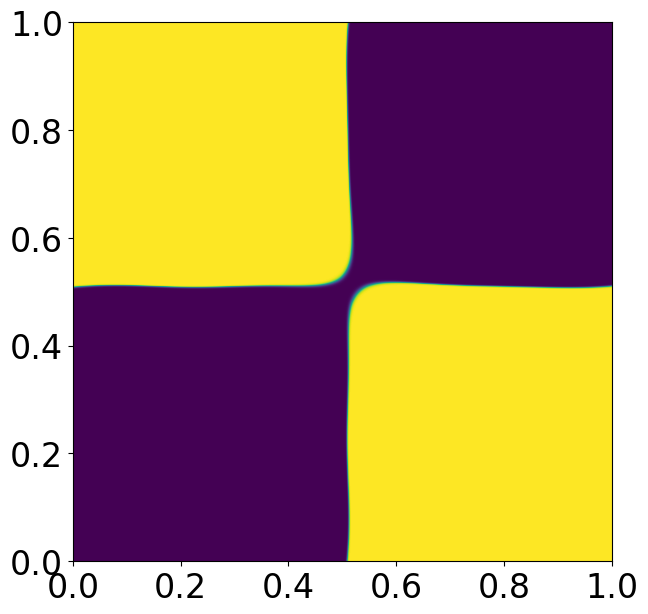
\includegraphics[width=\twoimagewidth]{new_figures/pet_50.png}
    \caption{Found graphon, $p=1/2$.}
    \label{fig:opt-pet-50}
  \end{subfigure}
  \begin{subfigure}{\twowidth}
    \centering
    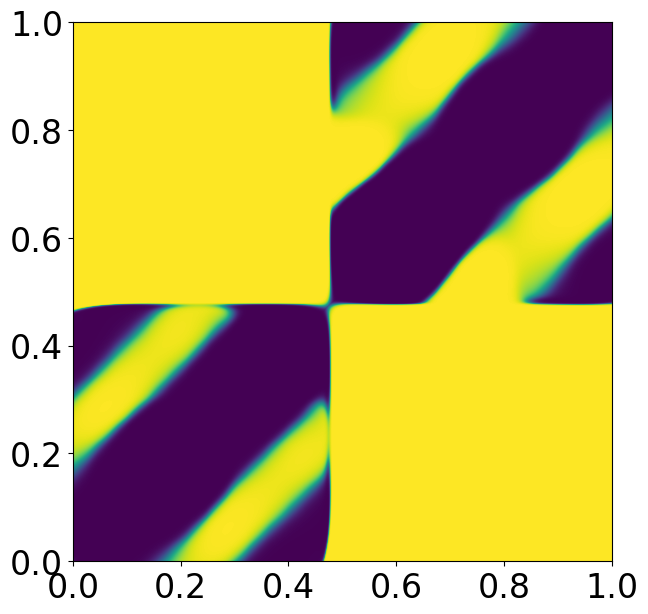
\includegraphics[width=\twoimagewidth]{new_figures/pet_67.png}
    \caption{Found graphon, $p=2/3$.}
    \label{fig:opt-pet-67}
  \end{subfigure}
  \begin{subfigure}{\twowidth}
    \centering
    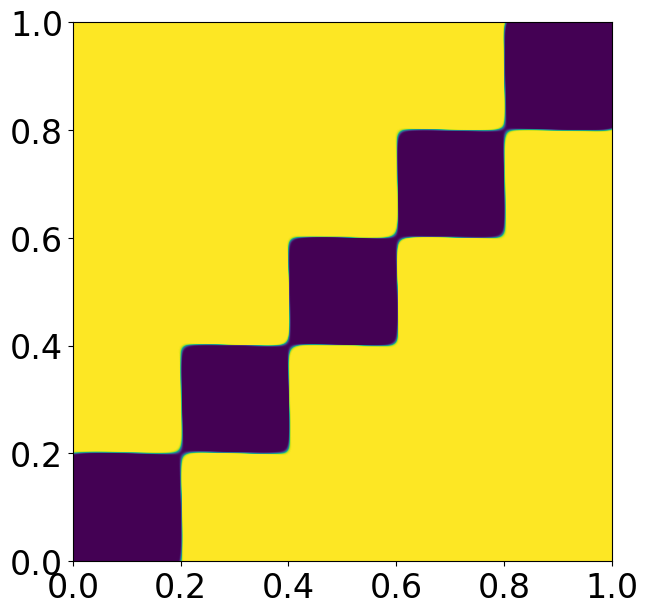
\includegraphics[width=\twoimagewidth]{new_figures/pet_80.png}
    \caption{Found graphon, $p=4/5$.}
    \label{fig:opt-pet-80}
  \end{subfigure}
  
  \begin{subfigure}{\twowidth}
    \centering
    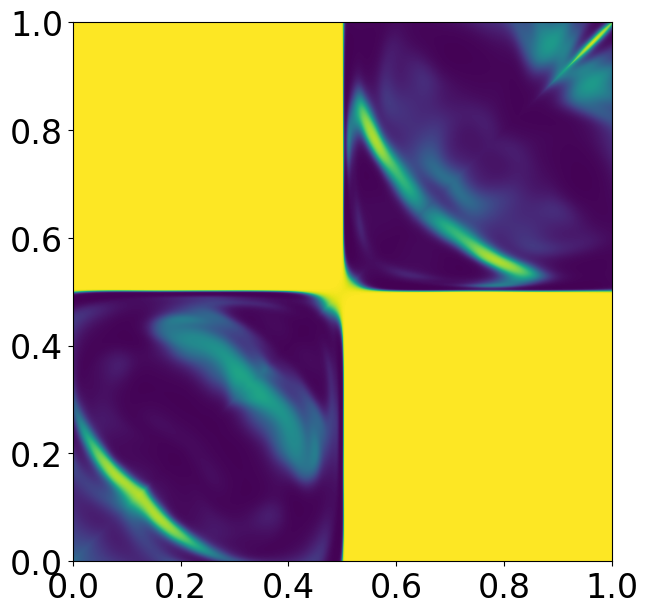
\includegraphics[width=\twoimagewidth]{new_figures/pet_57.png}
    \caption{Found graphon, $p=4/7$.}
    \label{fig:opt-pet-57}
  \end{subfigure}
  \begin{subfigure}{\twowidth}
    \centering
    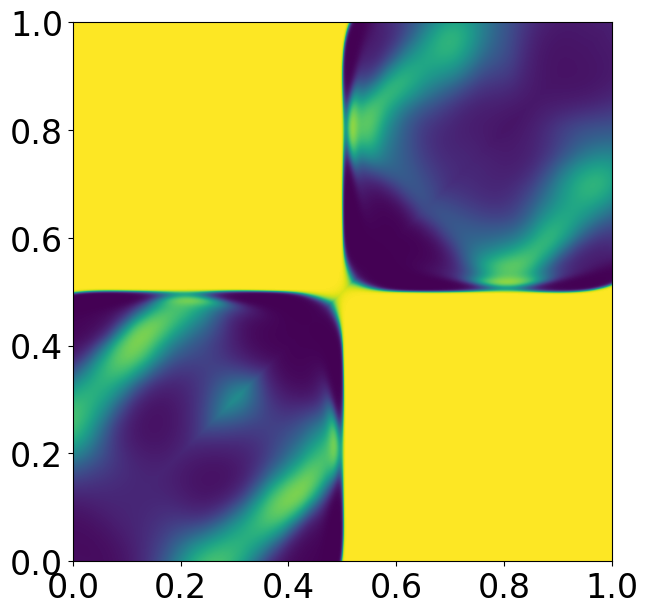
\includegraphics[width=\twoimagewidth]{new_figures/pet_62.png}
    \caption{Found graphon, $p=5/8$.}
    \label{fig:opt-pet-62}
  \end{subfigure}
  \begin{subfigure}{\twowidth}
    \centering
    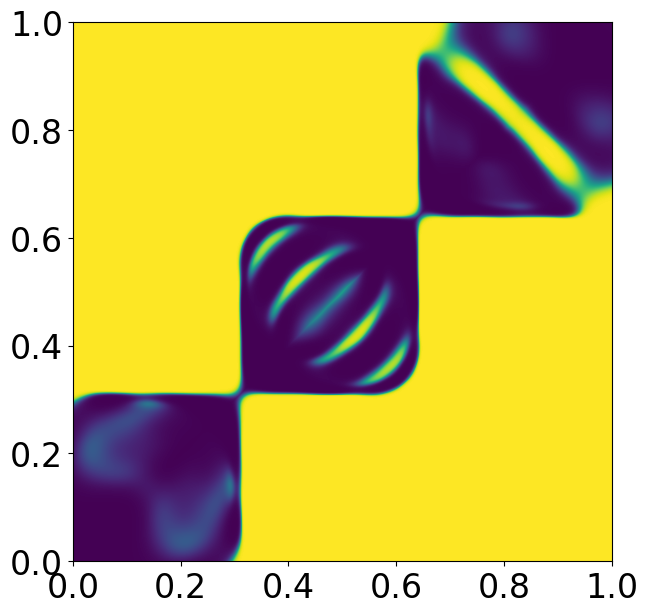
\includegraphics[width=\twoimagewidth]{new_figures/pet_71.png}
    \caption{Found graphon, $p=5/7$.}
    \label{fig:opt-pet-71}
  \end{subfigure}
  \caption{Graphons found for the Petersen graph density minimisation under the edge-density constraint $t(K_2, W)=p$.}
  \label{fig:petersenminimisation}
\end{figure}


\section{Details of Hand-crafted Graphons}
\label{sec:handcraftedgraphons}

In this section, we describe the hand-crafted graphons used as baselines in our experiments.
We consider edge densities satisfying $1 - 1/k < p < 1 - 1/(k+1)$, where $k$ is a positive integer.

The first two instances are graphons arising from the optimal solution to edge-density-constrained $K_3$ homomorphism-density minimisation.
We construct a complete $(k+1)$-partite graphon by partitioning $[0,1]$ into $(k+1)$ groups, $X_1, \ldots, X_{k+1}$, and defining
\[
  W_i(x_1, x_2) = \begin{cases}
    1 & \text{if } x_1 \in X_m,\ x_2 \in X_n,\ m \neq n
    \\
    0 & \text{if } x_1 \in X_m,\ x_2 \in X_m.
  \end{cases}
\]
We set $|X_1| = \cdots = |X_k| = x$ and $|X_{k+1}| = 1 - kx$, and choose $x$ to satisfy the edge-density constraint. This amounts to solving the quadratic equation
\[
  k(k-1)x^2 + 2k x (1-kx) = p.
\]
This quadratic has two solutions: one with $x > 1 - kx$ (denoted $W_1$) and one with $x < 1 - kx$ (denoted $W_2$). The first corresponds to the optimum for $K_3$ density minimisation.

The second instance is constructed by deleting edges from the complete $(k+1)$-partite graphon.
We partition the interval $[0,1]$ into $k$ groups $X_1, \ldots, X_k, X_{k+1}$ with $|X_1| = \cdots = |X_k| = |X_{k+1}| = 1/(k+1)$, and define
\begin{align*}
  W_3(x_1, x_2) &= \begin{cases}
    \frac{(k+1)p}{k} & \text{if } x_1 \in X_m,\ x_2 \in X_n,\ m \neq n
    \\
    0 & \text{if } x_1 \in X_m,\ x_2 \in X_m,
  \end{cases}
  \\
  W_4(x_1, x_2) &= \begin{cases}
    \frac{p (k+1)^2 - k^2 - k + 2}{2} & \text{if } x_1 \in X_1,\ x_2 \in X_2\ \text{or vice versa}
    \\
    0 & \text{if } x_1 \in X_m, x_2 \in X_m,
    \\
    1 & \text{otherwise}.
  \end{cases}
\end{align*}
For $1 - 1/k < p < 1 - 1/(k+1)$, both nontrivial edge probabilities above lie in $[0,1]$: their non-negativity follows from the lower bound on $p$, while $(k+1)p/k < 1$ and $\bigl(p(k+1)^2-k^2-k+2\bigr)/2 < 1$ follow from the upper bound.

Finally, the last graphon is the constant graphon $W(x_1, x_2) = p$.

We visualised $W_1, \ldots, W_4$ for $p=0.7$ in \Cref{fig:handcraftedgraphons}.

\begin{figure}
  \centering
  \begin{subfigure}{\twowidth}
      \centering
      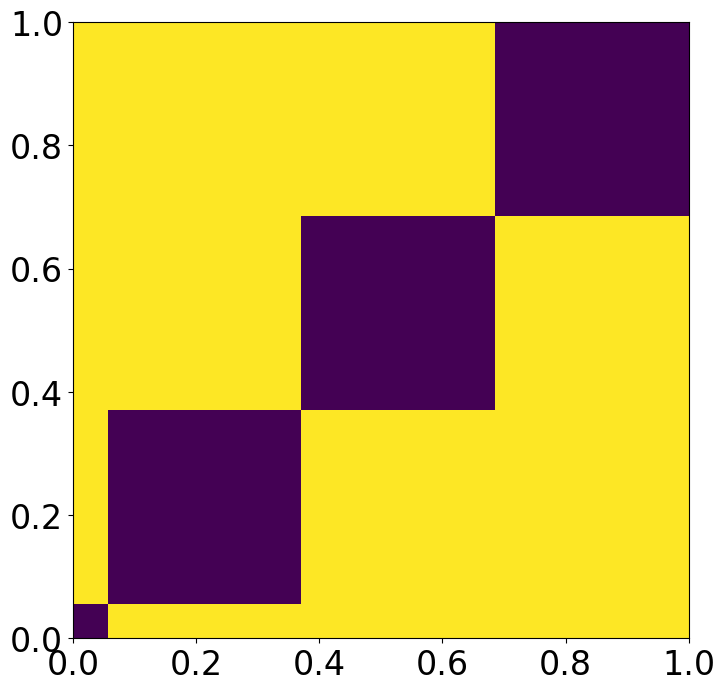
\includegraphics[width=\twoimagewidth]{figures/onesmall.png}
  \end{subfigure}
  \begin{subfigure}{\twowidth}
      \centering
      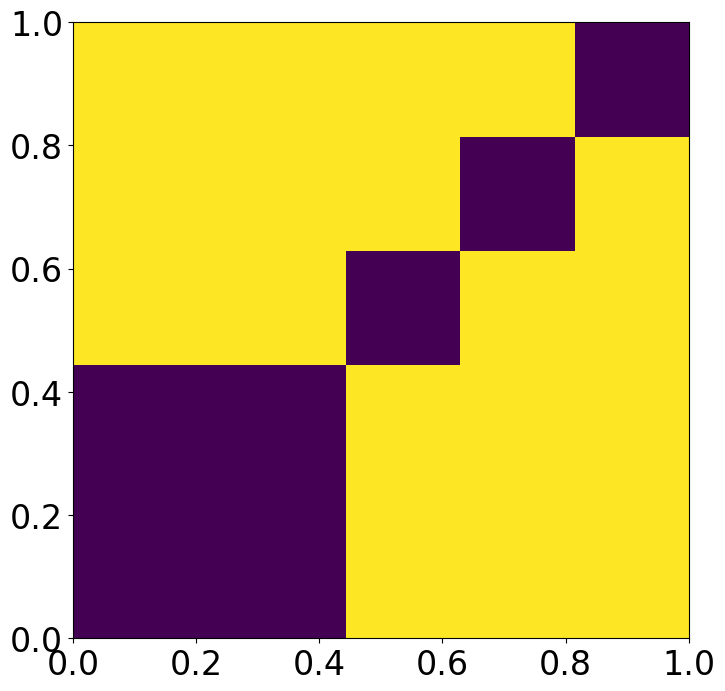
\includegraphics[width=\twoimagewidth]{figures/onelarge.png}
  \end{subfigure}
  
  \begin{subfigure}{\twowidth}
      \centering
      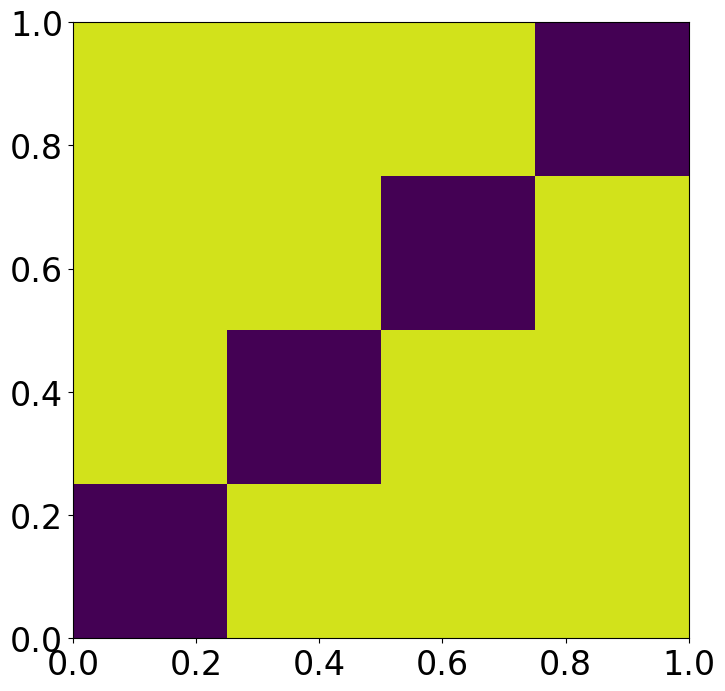
\includegraphics[width=\twoimagewidth]{figures/uniformless.png}
  \end{subfigure}
  \begin{subfigure}{\twowidth}
      \centering
      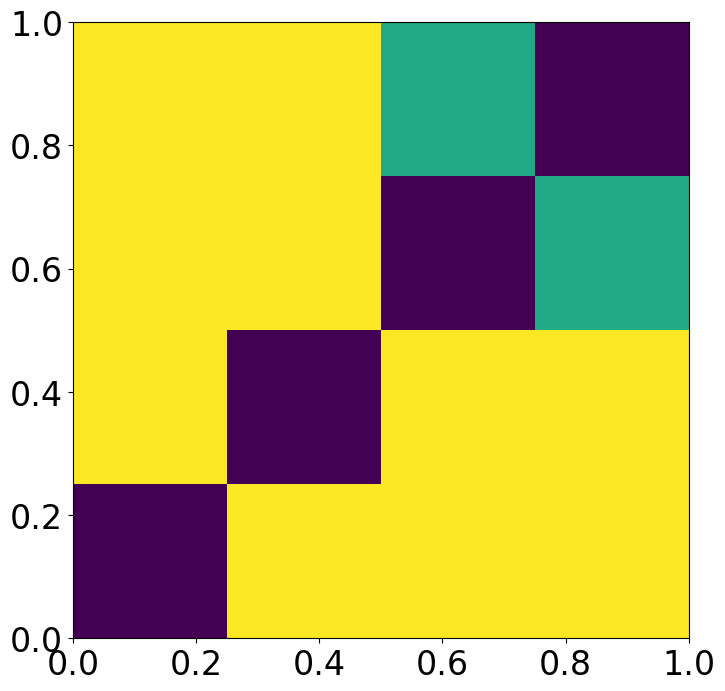
\includegraphics[width=\twoimagewidth]{figures/oneless.png}
  \end{subfigure}
  \caption{Hand-crafted graphons $W_1$ (top left), $W_2$ (top right), $W_3$ (bottom left), and $W_4$ (bottom right) with edge density $t(K_2, W)=0.7$.}
  \label{fig:handcraftedgraphons}
\end{figure}

\section{Ablation Study, Non-neural Baselines, and Multi-task Variant}
\label{sec:ablation}

\paragraph{Ablation Study.}
We perform an ablation study on triangle-density minimisation under the constraint $t(K_2,W)=7/9$, which is not of the form $1-1/k$ and admits multiple types of optima.
We consider four variants: (1) replacing our architecture with a ResNet that uses sinusoidal input encoding only in the first layer; (2) using a constant per-layer input encoding scale $s$; (3) enforcing the constraint via a regulariser; and (4) using a constant learning rate instead of cosine-annealing scheduling.
For fair comparison, we performed hyperparameter searches for the constant value of $s$ in (2), the strength of the regulariser in (3), and the constant learning rate in (4); we report the best run for each variant.
The graphons found by these variants are shown in \Cref{fig:ablationstudy} and quantitative results in \Cref{tab:ablationstudy}.
The ResNet variant (1) and the constant-scale variant (2) often fail to recover sharp, straight boundaries, consistent with a stronger bias toward smooth functions.
With the penalty-based constraint (3), the learnt graphon often violates fine structural details (e.g., the size of the smallest block).
Without cosine-annealing scheduling (4), the learnt graphon either fails to capture the multi-block structure (low learning rates) or exhibits less stable boundaries (high learning rates), highlighting the benefit of alternating between higher and lower learning rates.

\begin{table}[t]
  \centering
  \caption{$K_3$ densities in graphons found by our method and ablations for $K_3$ density minimisation under $t(K_2, W)=7/9$.  \label{tab:ablationstudy}}
  {\small
  \begin{tabular}{ll}
  \toprule
                     & $t(K_3, W)$ \\
  \midrule
  Ours                                     & $0.427215$ \\
  ResNet                                   & $0.428968$ \\
  Constant-scale $s$                       & $0.428190$ \\
  Regulariser                              & $0.434445$ \\
  Constant LR (low)                        & $0.430071$ \\
  Constant LR (high)                       & $0.431645$ \\
  \midrule
  SBM (256 blocks, fixed sizes)            & $0.428190$ \\
  SBM (5 blocks, trainable sizes)          & $0.429441$ \\
  SBM (64 blocks, trainable sizes)         & $0.429441$ \\
  Decision Tree                            & $0.455558$ \\
  Gradient Boosted Decision Tree                   & $0.454485$ \\
  \bottomrule
  \end{tabular}
  }
\end{table}

\begin{figure}[t]
  \centering
  \begin{subfigure}{0.155\textwidth}
    \centering
    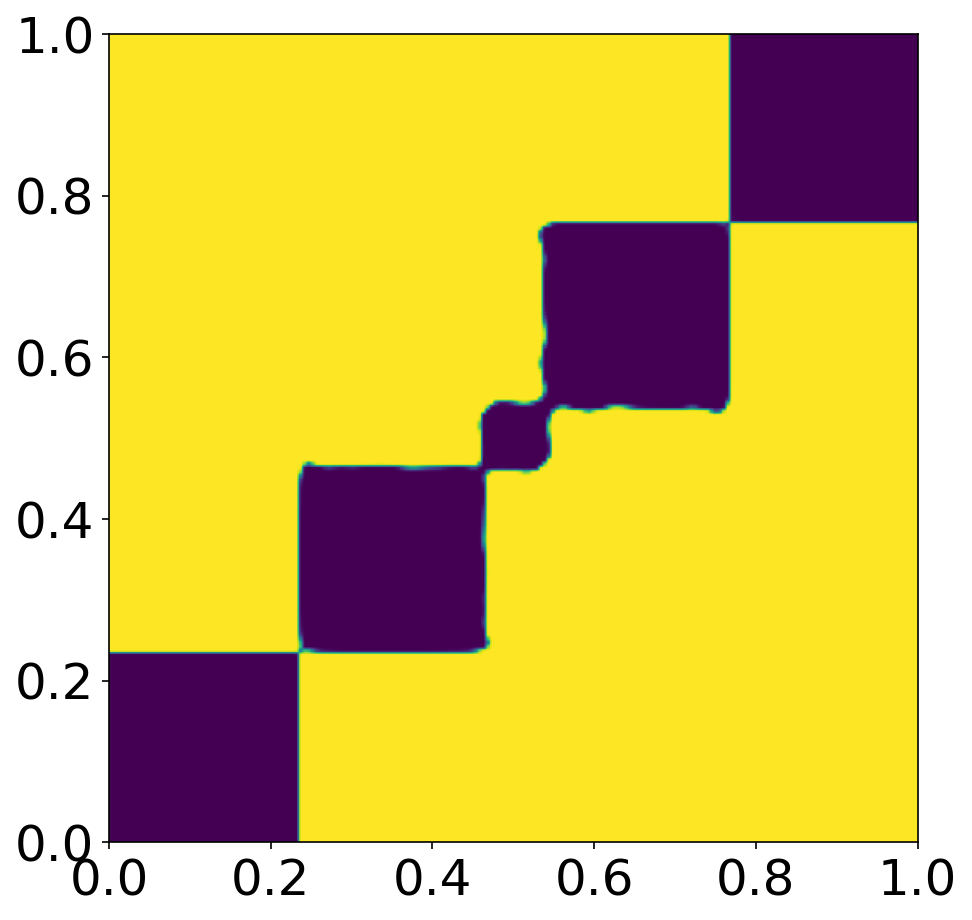
\includegraphics[width=1.1\textwidth]{figures/baseline.png}
    \caption{Our method.}
    \label{fig:baseline}
  \end{subfigure}
  \begin{subfigure}{0.155\textwidth}
    \centering
    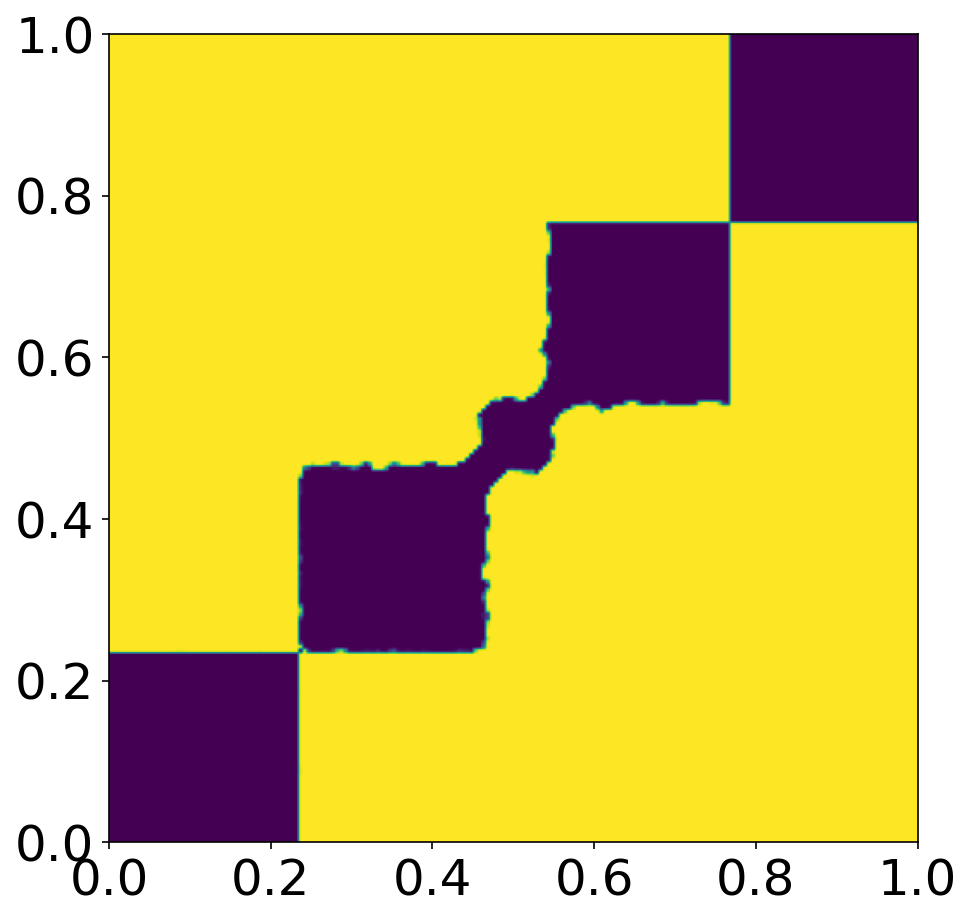
\includegraphics[width=1.1\textwidth]{figures/resnet.png}
    \caption{ResNet variant.}
    \label{fig:resnet}
  \end{subfigure}
  \begin{subfigure}{0.155\textwidth}
    \centering
    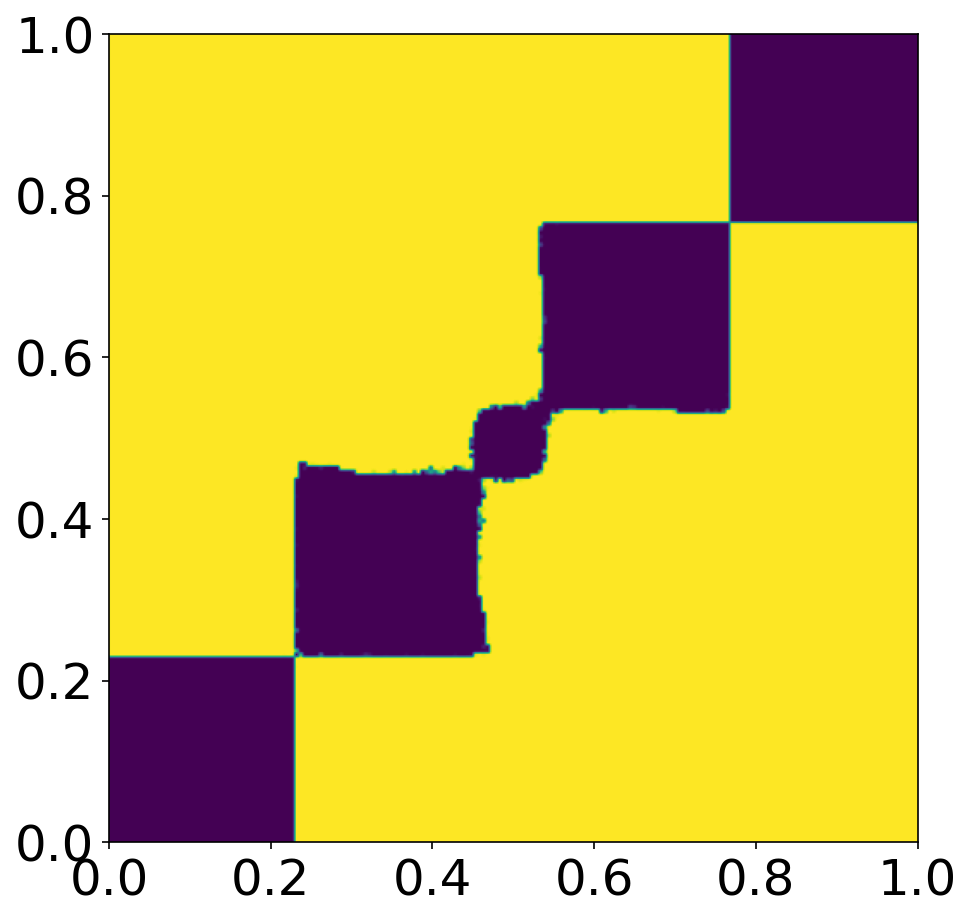
\includegraphics[width=1.1\textwidth]{figures/const4.png}
    \caption{Constant-scale~$s$.}
    \label{fig:const2}
  \end{subfigure}

  \begin{subfigure}{0.155\textwidth}
    \centering
    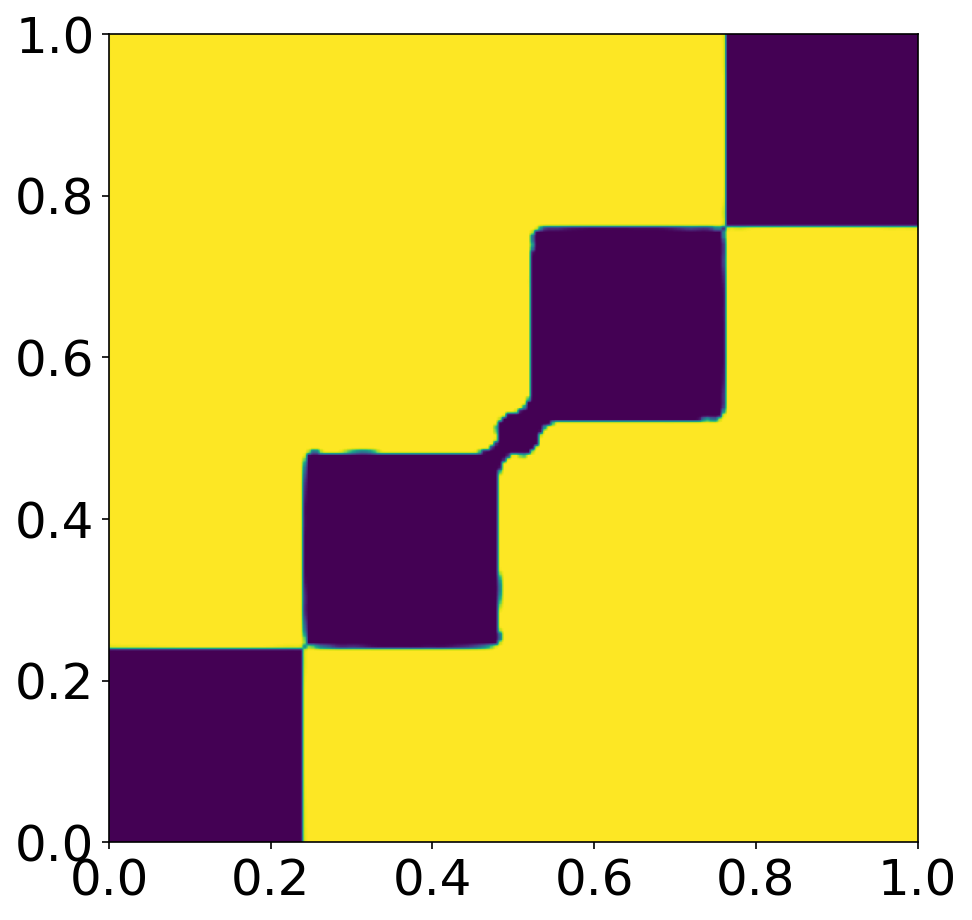
\includegraphics[width=1.1\textwidth]{figures/noconstraint.png}
    \caption{Regulariser.}
    \label{fig:noconsthighreg}
  \end{subfigure}
  \begin{subfigure}{0.155\textwidth}
    \centering
    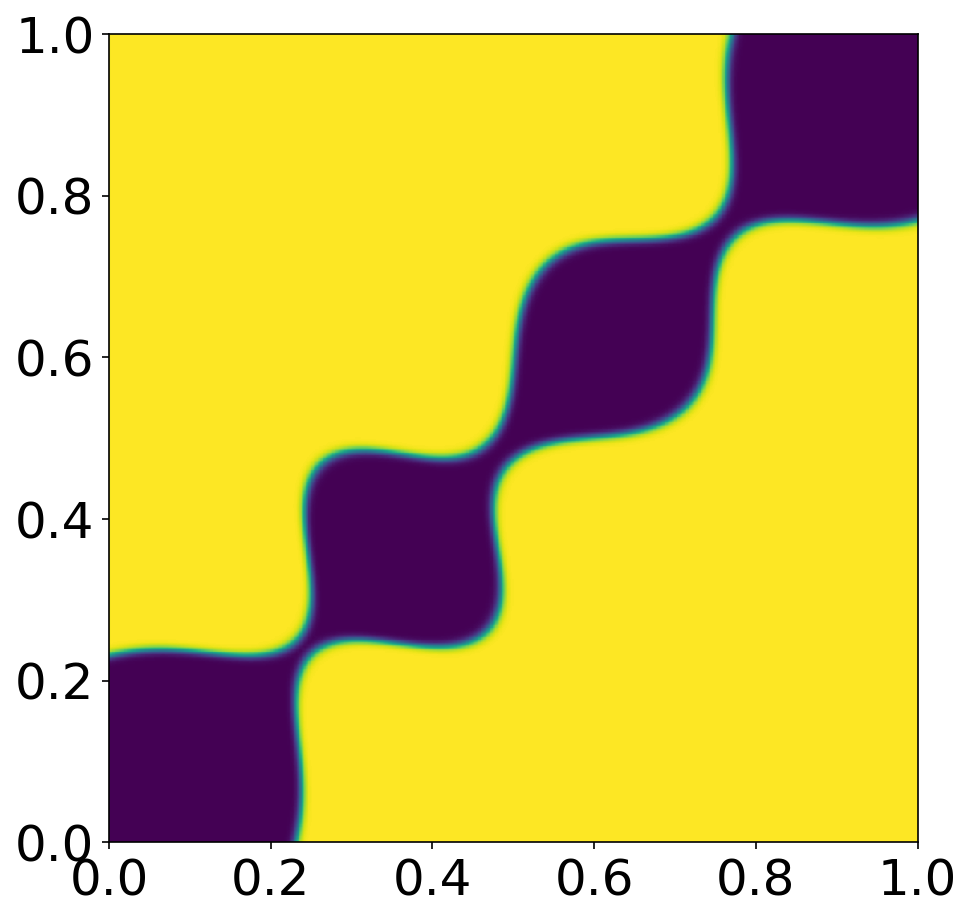
\includegraphics[width=1.1\textwidth]{figures/noscaling-lowlr.png}
    \caption{Const.~LR (low).}
    \label{fig:noscheduling-lowlr}
  \end{subfigure}
  \begin{subfigure}{0.155\textwidth}
    \centering
    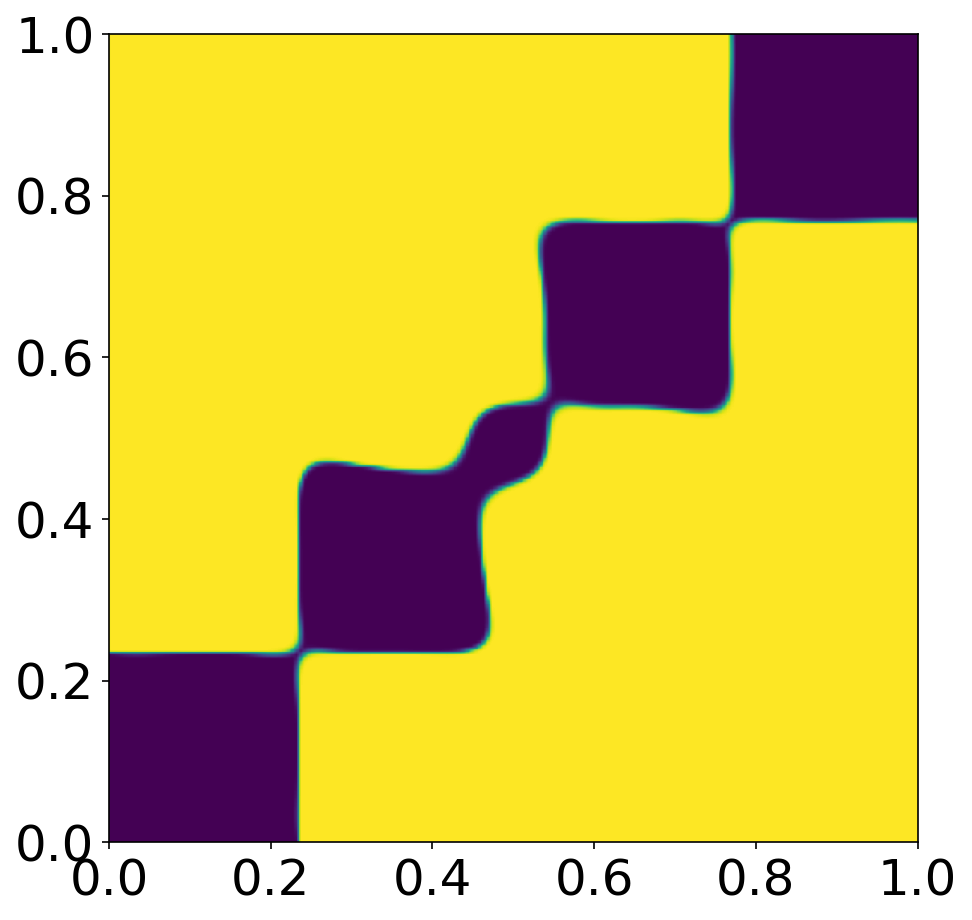
\includegraphics[width=1.1\textwidth]{figures/noscaling-highlr.png}
    \caption{Const.~LR (high).}
    \label{fig:noscheduling-highlr}
  \end{subfigure}
  \caption{Graphons found by our method and its ablations, for $K_3$ density minimisation under the constraint $t(K_2, W) = 7/9$.}
  \label{fig:ablationstudy}
\end{figure}

\paragraph{Non-neural Baselines.}
On the same triangle-density-minimisation task we evaluated four non-neural baselines tailored to step graphons: (a) a stochastic block model (SBM) with $256$ equal-sized blocks and trainable edge densities; (b) SBMs with $5$ blocks and $64$ blocks, with trainable edge densities and trainable block sizes; (c) a decision tree; and (d) a tree ensemble. Each baseline was run four times from independent random initialisations, and we report the best objective value across runs in \cref{tab:ablationstudy}. 
The SBMs with trainable block sizes collapsed to nearly constant graphons, suggesting a difficult optimisation landscape; the fixed-block SBM recovered a noisy multi-block structure; the tree-based baselines produced structured but qualitatively different graphons. All four baselines achieved worse objective values than every ablated variant of our architecture above, providing direct support for the choice of a neural representation in this setting.

\paragraph{Multi-task Variant.}
The main paper trains one network per $(H, p)$. To probe whether shared training across related tasks is viable, we ran a preliminary FiLM-conditioned architecture \citep{perez2018film} jointly trained over $p \in [1/2, 2/3]$ for $H = K_3$. The resulting network achieves absolute error at most $2.09 \times 10^{-4}$ and average absolute error $3.12 \times 10^{-5}$ relative to the known optimum, with $p$ sampled uniformly from $[1/2, 2/3]$. While limited to a single graph, this experiment indicates that shared training across related tasks can substantially reduce the per-instance burden of our framework, and we view a fuller multi-task / multi-graph treatment as a natural extension.

\end{document}

% This document was modified from the file originally made available by
% Pat Langley and Andrea Danyluk for ICML-2K. This version was created
% by Iain Murray in 2018, and modified by Alexandre Bouchard in
% 2019 and 2021 and by Csaba Szepesvari, Gang Niu and Sivan Sabato in 2022.
% Modified again in 2023 and 2024 by Sivan Sabato and Jonathan Scarlett.
% Previous contributors include Dan Roy, Lise Getoor and Tobias
% Scheffer, which was slightly modified from the 2010 version by
% Thorsten Joachims & Johannes Fuernkranz, slightly modified from the
% 2009 version by Kiri Wagstaff and Sam Roweis's 2008 version, which is
% slightly modified from Prasad Tadepalli's 2007 version which is a
% lightly changed version of the previous year's version by Andrew
% Moore, which was in turn edited from those of Kristian Kersting and
% Codrina Lauth. Alex Smola contributed to the algorithmic style files.
